\documentclass[12pt]{amsart}

\usepackage{tikz}
\usetikzlibrary{snakes}
\usepackage[colorlinks=true, linkcolor=blue, anchorcolor=blue, citecolor=blue, filecolor=blue, menucolor= blue, urlcolor=blue]{hyperref}
\usepackage{amsmath,amssymb,amsthm,amscd}
\usepackage{verbatim}
\usepackage{comment}
\usepackage{multirow}
\usepackage{mathtools}
\usepackage{enumitem}
\usepackage{pgf,tikz}
\usetikzlibrary{arrows}
\usepackage[normalem]{ulem}

\usepackage[margin=1in]{geometry} 

\numberwithin{equation}{section}

\newtheorem{theorem}{Theorem}[section]
\newtheorem{proposition}[theorem]{Proposition}
\newtheorem{lemma}[theorem]{Lemma}
\newtheorem{corollary}[theorem]{Corollary}
\newtheorem{problem}[theorem]{Problem}
\newtheorem{question}[theorem]{Question}
\newtheorem{conjecture}[theorem]{Conjecture}
\newtheorem*{theorem*}{Theorem}

\theoremstyle{definition}
\newtheorem{definition}[theorem]{Definition}
\newtheorem{notation}[theorem]{Notation}
\newtheorem{example}[theorem]{Example}
\newtheorem{remark}[theorem]{Remark}

\definecolor{MyDarkGreen}{cmyk}{0.7,0,1,0}

   
   

\begin{document}

\title[Line arrangements]{Line arrangements and configurations of points with an unusual geometric property}

\author{D.\ Cook II}
\address{Department of Mathematics and Computer Science\\
Eastern Illinois University\\
600 Lincoln Avenue\\
Charleston, IL 61920-3099 USA}
\email{dwcook@eiu.edu}

\author{B.\ Harbourne}
\address{Department of Mathematics\\
University of Nebraska\\
Lincoln, NE 68588-0130 USA}
\email{bharbour@math.unl.edu}

\author{J.\ Migliore} 
\address{Department of Mathematics \\
University of Notre Dame \\
Notre Dame, IN 46556 USA}
 \email{migliore.1@nd.edu}

\author{U.\ Nagel}
\address{Department of Mathematics\\
University of Kentucky\\
715 Patterson Office Tower\\
Lexington, KY 40506-0027 USA}
\email{uwe.nagel@uky.edu}

\begin{abstract} 
    The SHGH conjecture proposes a solution to the question of how many conditions a general union of fat points imposes on
    the complete linear system of curves in $\mathbb P^2$ of fixed degree $d$, and it is known to be true in many cases. We
    propose a new problem, namely to understand the number of conditions imposed by a general union of fat points on the
    incomplete linear system defined by the condition of passing through a given finite set of points $Z$ (not general). Motivated
    by work of Di Gennaro-Ilardi-Vall\`es and Faenzi-Vall\`es, we give a careful analysis for the case where there
    is a single general fat point, which has multiplicity $d-1$. There is an expected number of conditions imposed by this fat point, and we
    study those $Z$ for which this expected value is not achieved. We show, for instance, that if $Z$ is in linear general position
    then such unexpected curves do not exist.  We give criteria for the occurrence of such unexpected curves and describe the range
    of values of $d$ for which they occur. We also exhibit examples where the unexpected curve is even irreducible. Furthermore, we relate properties
    of $Z$ to properties of the arrangement  of lines dual to the points of $Z$. In particular, we obtain a new interpretation of
    the splitting type of a line arrangement. Finally, we use our results to establish a Lefschetz-like criterion for Terao's
    conjecture on the freeness of line arrangements.
\end{abstract}

\date{February 5, 2016}

\thanks{
{\bf Acknowledgements}: Harbourne was partially supported by NSA grant number  H98230-13-1-0213.
Migliore was partially supported by NSA grant number H98230-12-1-0204 and by Simons Foundation grant \#309556.
Nagel was partially supported by NSA grant number H98230-12-1-0247 and by Simons Foundation grant \#317096.
We thank A.\ Seceleanu, S.\ Tohananu and J. Vall\`es for their comments on this paper.}

\keywords{fat points, line arrangements, strong Lefschetz property, linear systems, stable vector bundle, splitting type}

\subjclass[2010]{14N20 (primary); 05E40, 14C20, 14F05 (secondary)}

\maketitle

\section{Introduction}

A fundamental problem in algebraic geometry is the study of the dimension of linear systems on projective varieties, and many tools have been developed by researchers to this end (e.g. the different versions of the Riemann-Roch theorem). It is usually the case that there is an {\em expected} dimension (or codimension), given by naively counting constants; understanding the  {\em special} linear systems, i.e., those whose actual dimensions are greater than the expected ones, is a subtle problem of substantial interest.

For example, consider the complete linear system $\mathcal V=\mathcal L_j$ of plane curves of degree $j$; its (projective) dimension is  $\binom{j+2}{2}-1$. For $j\geq m$,  the requirement that the curves all have multiplicity at least $m$ at a fixed point $P$ imposes $\binom{m+1}{2}$ linear conditions, and the   linear subsystem of all such curves indeed has codimension $\binom{m+1}{2}$ in $\mathcal V$,  so the actual and expected codimensions coincide. We will refer to this as the  linear subsystem of curves passing through a {\em fat point of multiplicity $m$}  supported at $P$. It is a very well-studied (but still open) problem to compute the dimension of the linear subsystem of $\mathcal L_j$ of curves of degree $j$ passing through a {\em general} set of $r$ fat points $P_1,\ldots,P_r$ with multiplicities $m_1,\dots, m_r$. The still open {\em SHGH Conjecture} gives a putative solution to this problem; we will recall  this conjecture in more detail below. 
When $m_1=\ldots=m_r=2$, results of Alexander-Hirschowitz not only confirm the SHGH Conjecture for those cases, but also solve the 
corresponding problem for double points in projective spaces of dimension greater than~2; however, little is known for fat points with arbitrary multiplicity in higher dimensions. 

Motivated by results in this paper described below, we propose a refinement of the above problem. That is, rather than beginning with $\mathcal V = \mathcal L_j$, we propose to begin with the linear system $\mathcal V= \mathcal L_{Z,j}$ of all plane curves of degree $j$  containing a fixed, reduced 0-dimensional scheme $Z$. We then impose the passage through a general set $X$ of fat points and ask for the dimension of the resulting linear subsystem.  The expected dimension depends only on the dimension of the homogeneous component $[I_Z]_j$ of degree $j$ of the ideal of $Z$ and the number of points of $X$, counted with multiplicity: each point of multiplicity $m$ is expected to impose $\binom{m+1}{2}$ independent conditions, as long as the expected dimension of the linear system is non-negative. 

The problem in this generality is currently inaccessible; the case that $X$ is an arbitrary finite general set of fat points and $Z=\varnothing$, for example, has only a conjectural solution, given by the still open SHGH Conjecture. So for this paper we begin a study of this problem by focusing on the first nontrivial case at the other extreme, namely, $X$ a single fat point  of multiplicity $j-1$ and $Z$  an arbitrary finite reduced set of points.
It is surprising (as the example of \cite{DIV} in the next paragraph shows) that already in this case, it is no longer true that the expected dimension is necessarily achieved, as it was when we began with $\mathcal V= \mathcal L_j$ (i.e., when $X$ is one fat point and $Z=\varnothing$). Since $Z$ is {\em not} assumed to be a general set of points, the problem obtains a new and central aspect, namely to understand how the geometry of $Z$ can affect the desired dimension. 
In this paper we  carefully analyze  this surprising behavior. Furthermore, we show that our results have interesting connections to the study of line arrangements. In particular, they give  new perspectives on Terao's freeness conjecture, including a generalization to non-free arrangements.

Our original inspiration came in two ways, from a paper of 
Di Gennaro, Ilardi, and Vall\`es  \cite{DIV}. 
The first was by an example of \cite{DIV}, in which
 they observe that the set of nine points in ${ \ensuremath{\mathbb{P}}}^2$  dual to 
 the so-called B3 arrangement has an unusual geometric property \cite[Proposition 7.3]{DIV}: For every point $P$ of the plane, there is a degree four curve passing through these nine points and vanishing to order three at  $P$. This is surprising because a naive dimension count suggests that the  linear system of curves of degree 4 containing the nine points and $3P$ should be empty except for a special locus of points $P$, but in fact it is nonempty for a general point~$P$. 

This led us to study finite sets of points 
$Z$ in the plane for which, for some integer $j$, the dimension of the linear system of plane
curves of degree $j+1$ that pass  through the points of $Z$ and have multiplicity $j$ at a general point $P$ is unexpectedly large. In this case, we say that $Z$ admits an \emph{unexpected curve} of degree $j+1$ (see Definition \ref{def:unexpected curve}). We establish a numerical criterion for the occurrence of unexpected curves. It involves two invariants. The first one, which arose already in the work of Faenzi and Vall\'es \cite{FV2}, we call the \emph{multiplicity index}  $m_Z$ of $Z$. It  is the least integer $j$ such that the linear system of degree $j+1$ forms vanishing at $Z + jP$ is not empty (see Definition \ref{def:mult ind}). 
The second invariant, which is new,  is $t_Z := \min \big\{j \ge 0 \; : \; h^0(\mathcal I_Z(j+1)) - \binom{j+1}{2} > 0 \big\}$ (see Definition \ref{def:tZ}). It depends only on the Hilbert function of $Z$.

It turns out that a set $Z$ of points can have unexpected curves of various degrees. To understand this range of degrees we introduce  another new invariant, $u_Z$, called the \emph{speciality index} of $Z$,  as the least integer $j$ such that the scheme $Z + j P$, where $P$ is a general point, imposes independent conditions on forms of degree $j+1$ (see Definition \ref{def:u_Z}). Our first main result (see Theorem~\ref{u_ZTheorem}) is: 

\begin{theorem}\label{mainThm1} $Z$ admits an unexpected curve if and only if $m_Z < t_Z$. Furthermore, in this case $Z$ has an unexpected curve of degree $j$ if and only if $m_Z < j \le u_Z$. 
\end{theorem}

In particular, the existence of an unexpected curve forces $Z$ to be \emph{generally special}, that is,  $m_Z < u_Z$. The converse, however, is not necessarily true: if $Z$ is generally special, it does not necessarily have an unexpected curve.
The introduction and study of generally special sets of points is a key step in establishing  our existence criterion for unexpected curves. Another key ingredient is the study of the dimension of the linear system of curves of degree $m_Z + 1$,  as $Z$ admits any unexpected curve if and only if this linear system contains an unexpected curve.  We show in Theorem~\ref{thm:dim is two} that the dimension of the linear system of degree $m_Z + 1$ curves  is always one, unless $u_Z = m_Z -1$. In the latter case, the dimension is two. It follows that any unexpected curve of degree $m_Z + 1$ is uniquely determined by $Z$ and the general point $P$. The mentioned dimension result also allows us to predict how the multiplicity index changes when one adds to $Z$ another general point $Q$ (see Proposition \ref{conj:change of dZ}). Furthermore, we use it to derive a criterion for when the linear system of degree $m_Z + 1$ curves through $Z + m_Z P$ consists of a unique \emph{irreducible} curve (see Corollary \ref{irred curve least deg}). 

Checking for the existence of unexpected curves  requires computing $m_Z$ and $t_Z$.
Since $t_Z$ depends only on the fixed reduced scheme $Z$, it is typically easy to compute. 
In contrast $m_Z$ is much harder to compute rigorously (although one can get evidence for its value
using randomly selected points $P$). Work of Faenzi and Vall\`es \cite{FV2} relates $m_Z$ to properties of
the arrangement of lines ${\mathcal{A}}_Z$ dual to the points of $Z$.

Recall that associated to any line arrangement ${\mathcal{A}}$ is a locally free sheaf ${\mathcal{D}}$ of rank two, called the derivation bundle. Restricted to a general line $L$, it splits as ${\mathcal{O}}_L (-a) \oplus {\mathcal{O}}_L (-b)$ with $a + b = |Z| -1$. The pair $(a, b)$, where $a \le b$, is called the \emph{splitting type} of ${\mathcal{D}}$ or ${\mathcal{A}}$. 
For ${\mathcal{A}}= {\mathcal{A}}_Z$,  let us denote by ${\mathcal{D}}_Z$ the associated derivation bundle. Then \cite[Theorem 4.3]{FV2}
shows that the number $a$ is equal to the multiplicity index $m_Z$. 
We extend this by showing that the multiplicity index $m_Z$ and the speciality index $u_Z$ satisfy the relation $m_Z + u_Z = |Z| - 2$ (see Corollary \ref{cor:uZ}), and thus
that $b=u_Z+1$. 

This allows us to translate our results about finite sets of points into statements on line arrangements. In the other direction, we use methods for studying line arrangements to determine multiplicity indices of sets of points. For example, we determine the multiplicity index and the speciality index of a set of points in linearly general position and conclude that it does not admit any unexpected curves (see Corollary \ref{cor:dZ lin gen position}).  
We also show that the set of points dual to the Fermat configurations of $3 t \ge 15$ lines admit unexpected curves of degrees $t+2.\ldots,2t-3$ (see Proposition \ref{FermatProp}). 
Furthermore, we exhibit a family of free line arrangements with the property that any of the dual sets of points admits a unique unexpected curve which is in fact  irreducible (see Proposition~\ref{prop:unexpected irr}).
\smallskip 

The second way that \cite{DIV} inspired us relates to a fundamental open problem in the study of hyperplane arrangements, namely, Terao's conjecture, which is open even for line arrangements. A line arrangement ${\mathcal{A}} = {\mathcal{A}} (f)$ is said to be \emph{free} if the Jacobian ideal of $f$ is saturated, where $f$ is the product of linear forms defining the lines in ${\mathcal{A}}$. Terao conjectured that freeness is a combinatorial property, that is, it depends only on the incidence lattice of the lines in ${\mathcal{A}}$. In \cite{DIV}, the authors give an equivalent version of Terao's conjecture in terms of Lefschetz properties. 
In trying to understand their proof we realized that some of the results used in \cite{DIV} to derive the claimed equivalence are not quite true as stated. We use our results on points to clarify and to adjust the needed results. For example, in Theorem~\ref{SLP condition} we show that it is the existence of an unexpected curve (rather than ${\mathcal{D}}_Z$ being unstable) that is equivalent to the failure of a certain Lefschetz property. We also establish that Terao's conjecture is equivalent to a Lefschetz-like condition (see Proposition \ref{prop:Terao equiv}). This allows us to show that the (adjusted) Lefschetz condition given in \cite{DIV} implies Terao's conjecture (see Corollary \ref{cor:suff Terao}). While we do not know if this condition is also necessary,  
we do establish that Terao's conjecture follows if one can show that the splitting type of a free line arrangement is a combinatorial property (see Corollary \ref{cor:type of free comb}). We wonder, if, in fact, the splitting type of an arbitrary line arrangement is determined by its incidence lattice. 
\smallskip 

We end the introduction with the more detailed discussion of the SHGH Conjecture which we promised above
in the context of the larger problem which frames the work we are doing here. 
Let $V = [R]_j$ be the vector space of degree $j$ forms in three variables, let $\mathcal L_j$ be its projectivization, and let $X = m_1 P_1 + \cdots m_r P_r$ be a fat point scheme supported on a set of $r$ points $P_1,\ldots,P_r$. Thus $X$ is defined by 
\[
I_X = I_{P_1}^{m_1} \cap \cdots \cap I_{P_r}^{m_r}.
\]
We say that $X$ {\it fails to impose the expected number of conditions} on $V$ (or on $\mathcal L_j$) if
\[
\dim_K [I_X]_j > \max \left \{0, \ \dim_K V - \sum_i \binom{m_i+1}{2} \right \} = 
\max \left \{0, \ \binom{j+2}{2}  - \sum_i \binom{m_i+1}{2} \right \}. 
\]

If the points $P_i$ are general, it is a well-known and difficult 
open problem to classify all $m_i$ and $j$ such that the subscheme
$X$ fails to impose the expected number of conditions on $V$, but a conjectural 
answer is given by the SHGH Conjecture \cite{segre, Ha1, G, Hi}. Segre's
version of the conjecture, which ostensibly gives only
a necessary criterion, is as follows.
\smallskip

\begin{conjecture}[SHGH Conjecture] For $X = m_1 P_1 + \cdots m_r P_r$ 
with  general points $P_i$, $X$ fails to impose the expected number 
of conditions on $V$ only if $[I_X]_j\neq 0$ but
the base locus of $[I_X]_j$ contains a non-reduced curve.\smallskip
\end{conjecture}

In fact, the SHGH Conjecture as stated above is equivalent to
versions \cite{Ha1, G, Hi} that not only provide an explicit and complete list of all 
$(m_1,\ldots,m_r)$ and $j$ for which $[I_X]_j$ conjecturally fails to 
impose independent conditions on $V$ but which also conjecturally
determine the extent to which the conditions fail to be independent.
Although we will not discuss the details here, we note that it took 
40 years \cite{refCM} to recognize that the partial characterization
as given above actually provides a full quantitative 
conjectural solution. 

Similarly, our focus here will be on identifying failures
of independence in a generalized context, with a long term
goal of obtaining a more complete characterization. The generalized 
context is that we consider the case that $V$ is a subspace of $R_j$, 
in particular, $V= [I_Z]_j$, where $Z$ is a fat point subscheme. Then 
the overall problem becomes:

\smallskip

\begin{problem}
  \label{prob:intro}
 Characterize and then classify all  triples $(Z,X,j)$
where $Z=c_1 Q_1+\cdots +c_s Q_s$ for distinct points $Q_i$, $X = m_1 P_1 + \cdots m_r P_r$
for general points $P_i$, such that $X$ fails to impose the expected number of conditions on $V = [I_Z]_j$.  
\end{problem}

If $Z$ is the empty set, then $V=[R]_j$, so this is addressed by the SHGH Conjecture. If $Z$ is reduced,  $r = 1$, and $j = m_1 + 1$, this becomes the problem of deciding the existence of an unexpected curve of degree $j$. Our results give the following answer: 

\begin{theorem}
   \label{thm:intro}
Let $Z \subset { \ensuremath{\mathbb{P}}}^2$ be a finite set of points whose dual is a line arrangement with splitting type $(a, b)$.  Let $P$ be a general point. Then the subscheme $X = m P$ fails to impose the expected number of conditions on  $V = [I_Z]_{m+1}$ if and only if 
\begin{itemize}
\item[(i)]  $a \le m \le b-2$; \quad and 

\item[(ii)] $h^1 ({\mathcal{I}}_{Z} (t_Z)) = 0$. 
\end{itemize} 
\end{theorem} 

\noindent
Notice that Condition (ii) is equivalent to the assumption $\dim_K [R/I_Z]_{t_Z} = |Z|$. 

It would be interesting to understand exactly for which sets $Z$ the above failure of imposing the expected number of conditions occurs. Furthermore, our results strongly suggest that finding  answers to Problem \ref{prob:intro} in other cases is worth investigating. 
\smallskip 

Our paper is organized as follows: In Section \ref{sec:mult ind} we introduce the basic invariants, establish some preliminary results, and state our criterion for the occurrence of unexpected curves. Section \ref{sec:proof criterion} is entirely geared towards establishing this criterion. Our further results on the invariants, dimensions of linear systems, and characterizations of generally special set of points are derived in Section \ref{sec:criteria}.   The connection to line arrangements is made in Section \ref{arrangement section}. In particular, we show Theorem \ref{thm:intro} there.  In Section \ref{sec:SLP} we introduce the Lefschetz properties and relate them to the existence of unexpected curves. The relation of the Lefschetz properties to Terao's freeness conjecture is made precise in Section \ref{sec:Terao}. 

\section{A Criterion for the Occurrence of Unexpected Curves} 
\label{sec:mult ind} 

Throughout, $K$ denotes an infinite field. We denote the homogeneous coordinate ring of ${ \ensuremath{\mathbb{P}}}^2$ over $K$ by $R = K[{ \ensuremath{\mathbb{P}}}^2]=K[x,y,z]$.
Given distinct points $P, P_1,\ldots,P_s\in{ \ensuremath{\mathbb{P}}}^2$ and an integer $a>0$, we denote by 
$Z=P_1+\cdots+P_s$ the scheme defined by the ideal $I_Z=I_{P_1}\cap \cdots \cap I_{P_s}\subseteq R$,
where where $I_{P_i}$ is the ideal generated by all forms that vanish at $P_i$, and by 
$X=Z+jP$ the scheme defined by the ideal $I_X=I_P^j\cap I_Z$. 
(In particular, $Z$ will always be nonempty.)
In each degree $t$, note that $\dim_K [I_X]_t \geq \dim_K [I_Z]_t-\binom{j+1}{2}$;
i.e., the forms in $[I_X]_t$ are obtained from those of $[I_Z]_t$ by imposing at most
$\binom{j+1}{2}$ linear conditions coming from $jP$. Typically, if $\dim_K [I_X]_t > \dim_K [I_Z]_t-\binom{j+1}{2}$ 
(i.e., if $jP$ imposes fewer than $\binom{j+1}{2}$ conditions on $[I_Z]_t$)
for a general point $P$, it is because $\dim_K [I_Z]_t<\binom{j+1}{2}$ and $\dim_K [I_X]_t = 0$.
For special choices of $Z$, however, it can happen that $jP$ imposes fewer than
$\binom{j+1}{2}$ conditions even though $P$ is general and $\dim_K [I_X]_t >0$.
We are interested in exploring this situation when the degree $t$ is $j+1$.
This motivates the following definition, where we denote the sheafification
of a homogeneous ideal $I$ by $\mathcal I$. Also, given a sheaf $\mathcal F$ on ${ \ensuremath{\mathbb{P}}}^2$, 
we will usually write $h^0({ \ensuremath{\mathbb{P}}}^2, {\mathcal F})$ simply as $h^0({\mathcal F})$.
Thus, for example, $\mathcal I_Z \otimes \mathcal I_P^j=\mathcal I_X$,
$h^0({ \ensuremath{\mathbb{P}}}^2, {\mathcal I}_Z(t))=h^0({\mathcal I}_Z(t))=\dim_K [I_Z]_t$ and 
$h^0({ \ensuremath{\mathbb{P}}}^2,(\mathcal I_Z \otimes \mathcal I_P^j)(t))=h^0((\mathcal I_X)(t))=\dim_K [I_X]_t$. 

\begin{definition}
    \label{def:unexpected curve}
We say that a reduced finite set of points $Z \subset { \ensuremath{\mathbb{P}}}^2$  {\em admits an unexpected curve} if there is an integer $j>0$ such that, 
for a general point $P$, $jP$ fails to impose the expected number of conditions on the linear system of curves of 
degree $j+1$ containing $Z$. That is, $Z$ admits an unexpected curve of degree $j+1$ if 
\begin{equation}
  \label{eq:unexpected}
h^0((\mathcal I_Z \otimes \mathcal I_P^j)(j+1)) > \max \left  \{ h^0(\mathcal I_Z(j+1)) - \binom{j+1}{2}, 0 \right \}.
\end{equation}
\end{definition}

\begin{remark}
While it certainly can be of interest to ask when different kinds of non-reduced schemes admit ``unexpected curves" of this sort, in this paper we are concerned only with the case where $Z$ is reduced. Thus we assume from now on that $Z$ is a reduced, zero-dimensional subscheme of $\mathbb P^2$ whose degree is at least two  and will not repeat this throughout the paper.
\end{remark}

\begin{remark} \label{interesting}
If $0\leq j\leq1$ and $P$ is general, then $h^0((\mathcal I_Z \otimes \mathcal I_P^j)(j+1)) > 0$ implies
$h^0((\mathcal I_Z \otimes \mathcal I_P^j)(j+1)) = h^0(\mathcal I_Z(j+1)) - \binom{j+1}{2}\geq 0$.
Thus unexpected curves must have degree at least 3. 
\end{remark}

\begin{example}\label{FanoExample}
By Remark \ref{interesting}, the least degree for which an unexpected curve can occur is 3. 
We now show that unexpected curves of degree 3 can occur. 
Although the occurrence of unexpected curves is not purely a characteristic $p>0$ phenomenon
(later we will give examples in characteristic 0), we believe 2 is the only characteristic for which
an unexpected curve of degree 3 can occur. In any case, for this example
we assume $K$ to have characteristic 2, and for simplicity we assume $K$ is infinite. 
For this example, we show that \eqref{eq:unexpected} holds with $j+1=3$ and with the right hand side of \eqref{eq:unexpected} being 0.
Take $Z$ to be the seven points whose homogeneous coordinates $[a:b:c]$ consist of just zeroes and ones.
Note that the points are the points of the Fano plane and that any line through two of them goes through a third.
There are only seven such lines, and they are projectively dual to the seven points.
Let $P=[\alpha:\beta:\gamma]\in { \ensuremath{\mathbb{P}}}^2$ be a general point. One can check that
$Z$ imposes independent conditions on cubics (in fact, 
$I_Z=(yz(y + z),xz(x + z),xy(x + y))$). Since $Z+2P$ imposes 10 conditions,
one would expect that there would not be a cubic containing $Z$ having a double point at $P$.
But one can easily check that $F=\alpha^2yz(y + z)+\beta^2xz(x + z)+\gamma^2xy(x + y)$ defines a curve $C$ 
(reduced and irreducible in fact) which
is singular at $P$ and hence $C$ is an unexpected curve of degree 3 for $Z$.
\end{example}

In order for $Z$ to have an unexpected curve of some degree $j+1$,
it must be true that $[I_{Z+jP}]_{j+1}\neq0$. Thus it is worth looking for the 
least $j$ such that this holds. We will use this quantity to give 
a criterion for the occurrence of unexpected curves.

\begin{definition}[{\cite[Definition 4.1]{FV2}}]
    \label{def:mult ind}
(i) Given a point $P \notin Z$, we call 
\[
m_{Z, P} = \min\{j \ge 0 : h^0((\mathcal I_Z \otimes \mathcal I_P^j)(j+1)) > 0\}
\]    
the \emph{multiplicity index of $Z$ with respect to $P$}. 

(ii) By semicontinuity, fixing $Z$ and $j$, the integer $h^0((\mathcal I_Z \otimes \mathcal I_P^j)(j+1))$ 
is the same for all \emph{general} points $P \notin Z$ (and its value is the minimum value of
$h^0((\mathcal I_Z \otimes \mathcal I_P^j)(j+1))$ among points $P\notin Z$). Thus, for a general point $P$, 
\[
m_Z = m_{Z, P} 
\] 
is independent of the choice of $P$ and 
is said to be the \emph{multiplicity index of $Z$}.
\end{definition} 

We note that $m_{Z,P}$ exists for each point $P\notin Z$, since
it is easy to see that \linebreak $h^0((\mathcal I_Z \otimes \mathcal I_P^j)(j+1)) > 0$ holds
for all $j\geq \max\{0,|Z|\}$ (pick $j$ lines through $P$ which also 
go through the $|Z|$ points of $Z$), and hence $m_{Z,P}\leq \max\{0,|Z|\}$.
We also note that $h^0((\mathcal I_Z \otimes \mathcal I_P^j)(j+1))$ is a nondecreasing function of $j$,
since we have an injection $[I_Z \cap I_P^j]_{j+1}\to [I_Z \cap I_P^{j+1}]_{j+2}$
given by multiplication by any linear form $\ell$ vanishing at $P$.
Thus if $h^0((\mathcal I_Z \otimes \mathcal I_P^j)(j+1))=0$, then $m_Z>j$. The following exact sequence makes these observations more precise.  

\begin{lemma}
    \label{lem:exact sequence}
Let $Z \subset { \ensuremath{\mathbb{P}}}^2$ be a finite set of points, and let $P \in { \ensuremath{\mathbb{P}}}^2$  be any point that is not in $Z$.  Then, for every integer $j > 0$,  multiplication by a general linear form $\ell \in I_P$ on $R/I_{Z + j P}$ induces  an exact sequence  of graded $R$-modules
\begin{equation} 
    \label{eq:exact sequence}
0 \to (R/I_{Z + (j -1)  P}) (-1) \to  R/I_{Z + j P} \to R/(I_{Z + j P}, \ell) \to 0. 
\end{equation}
\end{lemma}

\begin{proof}
Since $P$ is not in $Z$ by assumption, we get $I_Z : \ell = I_Z$. Moreover, we have $I_P^{j} : \ell = I_P^{j-1}$. Now the claim follows. 
\end{proof}

As a consequence we see in particular that any finite set  $Z$ of points can have at most two  independent unexpected  curves of degree $m_Z + 1$. More generally, one has. 

\begin{lemma} 
   \label{lem:dim estimate}
Let $Z \subset { \ensuremath{\mathbb{P}}}^2$ be a finite set of points, and let $P \in { \ensuremath{\mathbb{P}}}^2$  be any point that is not in $Z$.     
Then 
\[
1 \le h^0((\mathcal I_{Z + m_Z P}(m_Z+1))  \le 2. 
\]
\end{lemma}

\begin{proof} Let $\ell$ be a a general linear form in  $I_P$. 
For ease of notation, set $m = m_Z$. The definition of $m$ gives 
\[
\dim_K [R/I_{Z + (m -1)  P}]_m = \binom{m+2}{2}  \quad \text{ and } \quad  \dim_K [R/I_{Z + m P}]_{m+1} < \binom{m+3}{2}.  
\]
Hence, Sequence \eqref{eq:exact sequence} with $j = m$ yields $\dim_K [R/(I_{Z + m P}, \ell)_{m+1} \le m+1$. Note that the ideal $(I_P^m, \ell)$ is generated by a regular sequence of two elements with degrees one and $m$, respectively. Therefore, we obtain the following estimates
\[
m = \dim_K [R/(I_P^m, \ell)]_{m+1} \le \dim_K [R/(I_{Z + m P}, \ell)_{m+1} \le m+1. 
\]
Using Lemma \ref{lem:exact sequence}, we conclude 
\[
\binom{m+3}{2} -  2 \le \dim_K [R/I_{Z + m P}]_{m+1} \le  \binom{m+3}{2} - 1, 
\]
which is equivalent to the assertion. 
\end{proof}  

Our criterion for the existence of unexpected curves will involve an additional quantity; it arises in 
the right hand side of \eqref{eq:unexpected}. It is also useful in giving
an upper bound on $m_Z$, better than the one above.

\begin{definition}
   \label{def:tZ}
For a reduced scheme $Z \subset { \ensuremath{\mathbb{P}}}^2$ consisting of a finite set of points, set 
\[
t_Z = \min \Big\{j \ge 0 \; : \; h^0(\mathcal I_Z(j+1)) - \binom{j+1}{2} > 0 \Big\}. 
\]
\end{definition} 

To see that $t_Z$ exists, it is helpful to rewrite $t_Z$ using the Hilbert function 
$h_Z: { \ensuremath{\mathbb{Z}}} \to { \ensuremath{\mathbb{Z}}}$ of $Z$, defined as $h_Z (j) = \dim_K [R/I_Z]_j$. 

\begin{lemma}
  \label{lem:rewrite rhs} For each integer $j \ge 0$ we have:

\begin{itemize}
\item[(a)] 
$\displaystyle h^0(\mathcal I_Z(j+1)) - \binom{j+1}{2} = 2 j + 3 - h_Z (j+1)$;

\item[(b)] 
$\displaystyle h^1(\mathcal I_{Z+j P} (j +1)) = h^0(\mathcal I_{Z+j P} (j+1)) + |Z| - (2j +3)$.

\end{itemize}
\end{lemma}

\begin{proof}
Part (a) is immediate from the facts that  $h^0(\mathcal I_Z(j+1)) = \binom{j+3}{2} - h_Z (j+1)$ and 
$\binom{j+3}{2} - \binom{j+1}{2} = 2 j+3$. Then part (b) follows from the exact sequence
\[
\begin{array}{ll}
0 \rightarrow H^0(\mathcal I_{Z+j P} (j+1)) \rightarrow H^0(\mathcal O_{\mathbb P^2} (j +1) \rightarrow H^0(\mathcal O_{Z + j P}(j+1)) \\ \\
\hspace{4in} \rightarrow H^1 (\mathcal I_{Z + j P}(j+1)) \rightarrow 0.
 \end{array}
\]
\end{proof}

\begin{corollary}\label{mz<tzCor}
Let $Z \subset { \ensuremath{\mathbb{P}}}^2$ be a reduced scheme consisting of a finite set of points. Then
$0\le m_Z\leq t_Z \le \left \lfloor \frac{|Z| -1}{2} \right \rfloor$.

Moreover, $t_Z = \left \lfloor \frac{|Z| -1}{2} \right \rfloor$ if and only if $h_Z (t_Z) = |Z|$. 
\end{corollary}

\begin{proof}
Since the Hilbert function of $Z$ is at most $|Z|$, by Lemma \ref{lem:rewrite rhs} 
we have
\[
h^0(\mathcal I_Z(j+1)) - \binom{j+1}{2} = 2 j + 3 - h_Z (j+1)\geq 2j+3-|Z|.
\]
Thus $t_Z$ is always defined 
and in fact $t_Z \le \left \lfloor \frac{|Z| -1}{2} \right \rfloor$. 
Since for any $P\notin Z$ we have
$h^0(\mathcal I_Z \otimes \mathcal I_P^{t_Z})(t_Z+1))\geq h^0(\mathcal I_Z(t_Z+1)) - \binom{t_Z+1}{2}>0$,
we see that $0\leq m_Z\leq m_{Z,P}\leq t_Z$. 

The above equality shows  that 
\[
t_Z = \min \{j \ge 0 \; : \; h_Z (j+1) \le 2 j +2 \}. 
\]
Now the characterization of the maximum value of $t_Z$ follows. 
\end{proof}

\begin{example}
   \label{rem:tZ}
Here we evaluate $t_Z$ exactly when $Z$ lies on a curve of low degree.
\begin{enumerate}
\item[(i)] The definition immediately gives that $t_Z = 0$ if and only if the points of $Z$ are collinear,
so in this case $t_Z$ is as small as possible, and we also have $m_Z=t_Z$.
\item[(ii)] If $Z$ lies on an irreducible conic, then  it is not hard to check that $t_Z = \left \lfloor \frac{|Z| -1}{2} \right \rfloor$,
so in this case $t_Z$ is as large as possible. Moreover, we again have $m_Z=t_Z$. (By Bezout's Theorem,
any form of degree $t_Z$ vanishing on $Z$ must be divisible by the form defining the conic. But the quotient
then has degree $t_Z-2$, which therefore cannot vanish to order $t_Z-1$ at a general point $P$. Thus $m_Z>t_Z-1$.)
\end{enumerate}
\end{example}

Our criterion involves one more quantity. In order for $Z$ to have an unexpected curve of degree $j+1$,
it must be the case for a general point $P$ that $Z+jP$ does not impose independent conditions on forms
of degree $j+1$, so the least $j$ for which the conditions are independent is of interest.

\begin{definition}\label{def:u_Z}
Let $Z$ be a reduced finite subscheme of ${ \ensuremath{\mathbb{P}}}^2$ and let $P$ be a general point.
Say that $Z$ is \emph{generally special} if $Z+m_ZP$ does 
not impose independent conditions on forms of degree $m_Z+1$, and we define the \emph{speciality index of $Z$} to be 
\[
u_Z = \min \{ j \geq 0 :  h^1({ \ensuremath{\mathbb{P}}}^2,\mathcal I_{Z+jP}(j+1))=0 \} ;
\]
i.e., $u_Z$ is the least integer $j$ such that $Z+jP$ imposes independent conditions on forms of degree $j+1$.
\end{definition}

We show in Lemma \ref{lem:uZ estimate} that $u_Z$ is well-defined, that is, $u_Z$ is finite. 
An interpretation of the speciality index in the context of line arrangements in $\mathbb P^2$   
will be given in Section~\ref{arrangement section}. 

The following observation shows that $u_Z$ can also be characterized as 
\[
u_Z = \max \{j \in { \ensuremath{\mathbb{Z}}} \; : \; h^1({ \ensuremath{\mathbb{P}}}^2,\mathcal I_{Z+jP}(j)) \neq 0 \}. 
\]
 
\begin{lemma}
   \label{cor:uZ implies}
Let $Z \subset { \ensuremath{\mathbb{P}}}^2$ be a finite set of points, and let $P \in { \ensuremath{\mathbb{P}}}^2$  be any point that is not in $Z$. Then  one has   
\[
 h^1({ \ensuremath{\mathbb{P}}}^2,\mathcal I_{Z+jP}(j+1))=0 \quad \text{ whenever } j \ge u_{Z, P},   
\]
where $u_{Z, P}  =  \min \{ j \geq 0 :  h^1({ \ensuremath{\mathbb{P}}}^2,\mathcal I_{Z+jP}(j+1))=0 \}$. 
\end{lemma} 

\begin{proof}
We use induction on $j$. If $j = u_{Z, P}$, the claim is true by definition of $u_{Z, P}$. Let $j > u_{Z, P}$. 
Let $\ell \in I_P$ be a general linear form. Then the saturation of $(I_{Z + jP}, \ell)$ is 
$(I_P^j, \ell) = (\ell, f)$ for some form $f \in I_P^j$. Denote by $Y$ the complete intersection defined by this ideal. 

Consider now the following part of the cohomology sequence induced by Sequence \eqref{eq:exact sequence}
\[
H^1 ({ \ensuremath{\mathbb{P}}}^2,\mathcal I_{Z+(j-1)P}(j)) \to H^1 ({ \ensuremath{\mathbb{P}}}^2,\mathcal I_{Z+(P}(j+1)) \to  H^1 ({ \ensuremath{\mathbb{P}}}^2,\mathcal I_Y (j+1)). 
\] 
The induction hypothesis gives that the group on the left-hand side is zero. Since the regularity of $Y$ equals $j$, the group on the right-hand side vanishes as well. It follows that $H^1 ({ \ensuremath{\mathbb{P}}}^2,\mathcal I_{Z+(P}(j+1)) = 0$, as desired. 
\end{proof} 

We now give an explicit upper bound on $u_{Z}$. 

\begin{lemma}
   \label{lem:uZ estimate}
Let $Z$ be a set of $s$ points in ${ \ensuremath{\mathbb{P}}}^2$, and let $P \in { \ensuremath{\mathbb{P}}}^2$ be a point that is not on any line through two of the points of $Z$.     Then $H^1({ \ensuremath{\mathbb{P}}}^2,\mathcal I_{Z+(s-2)P}(s-1)) = 0$. 
\end{lemma}

\begin{proof} 
We have to show that $Z + (s-2)P$ imposes $s + \binom{s-1}{2}$ conditions to the linear system of plane curves of degree $s-1$. Clearly $(s-2)P$ imposes $\binom{s-1}{2}$ conditions (since the regularity of $(s-2)P$ is $s-1$), so we want to show that the points of $Z$ impose $s$ independent conditions on the linear system, $\mathcal L$, of plane curves of degree $s-1$ vanishing to order $s-2$ at $P$. It is enough to show that given any point $Q$ of $Z$ there is a curve of degree $s-1$ vanishing to order $s-2$ at the general point $P$ and vanishing at each point of $Z \backslash \{Q\}$, but not vanishing at $Q$. This can be done (for instance) with a suitable union of $s-1$ lines, each joining $P$ and a point of $Z \backslash \{Q\}$.
\end{proof}

\begin{corollary}\label{u_ZCor}
Let $Z$ be a reduced finite subscheme of ${ \ensuremath{\mathbb{P}}}^2$. 

\begin{itemize}

\item[(a)] $u_Z\leq |Z|-2$, with equality if and only if the points of $Z$ lie on a line.

\item[(b)] If $Z$ is generally special, then $m_Z\leq t_Z\leq u_Z$, where one of the inequalities is strict.
\end{itemize}
\end{corollary}

\begin{proof}
Let $s = |Z|$.
If $P \in { \ensuremath{\mathbb{P}}}^2$ is a general point, then Lemma \ref{lem:uZ estimate} applies and shows $u_Z \leq |Z|-2$.

If the points of $Z$ lie on a line $\ell$ then any curve of degree $\leq s-2$ containing $s-1$ points of $Z$ must also contain the last point, so curves of degree $\leq s-2$ do not separate points of $Z$, and hence $u_Z = |Z|-2$. 

Conversely, assume that not all points of $Z$ lie on a line. We wish to show that $u_Z \leq s-3$, i.e. that $h^1(\mathcal I_{Z + (s-3)P} (s-2)) = 0$. 
Let $Q$ be any point of $Z$. We wish to find a curve of degree $s-2$ vanishing to order $s-3$ at $P$ and containing all the points of $Z \backslash \{Q\}$. This will follow from the above construction provided we can show that there is a line $\ell$ containing two points of $Z \backslash \{Q\}$ but not containing $Q$. Suppose this is not the case. Then the line joining any two points of $Z \backslash \{Q\}$ must also contain $Q$. Let $A,B$ be two points of $Z \backslash \{Q\}$ and let $\ell$ be the line spanned by $A$ and $B$, so $Q \in \ell$. Let $C$ be any point of $Z \backslash \{A,B,Q \}$. The line joining $C$ and $A$ also contains $Q$, so it must be $\ell$. In this way we see that all points of $Z$ must lie on $\ell$, contradicting our assumption.

Finally, if $Z$ is generally special, then $h^1({ \ensuremath{\mathbb{P}}}^2,\mathcal I_{Z+m_ZP}(m_Z+1))>0$ by definition,
hence $u_Z > m_Z$. But $h^0({ \ensuremath{\mathbb{P}}}^2,\mathcal I_{Z+m_ZP}(m_Z+1))>0$, so $u_Z> m_Z$
implies 
\[
h^0({ \ensuremath{\mathbb{P}}}^2,\mathcal I_{Z+u_ZP}(u_Z+1)) \geq h^0({ \ensuremath{\mathbb{P}}}^2,\mathcal I_{Z+m_ZP}(m_Z+1))>0 
\]
(just add lines through $P$ to get from $m_Z$ to $u_Z$) with $h^1({ \ensuremath{\mathbb{P}}}^2,\mathcal I_{Z+u_ZP}(u_Z+1))=0$. Since $Z + u_Z P$ imposes independent conditions on curves of degree $u_Z+1$, clearly $Z$ alone does as well. Hence
\[
\begin{array}{rcl}
h^0({ \ensuremath{\mathbb{P}}}^2,\mathcal I_Z(u_Z+1))-\binom{u_Z+1}{2} & = & \binom{u_Z+3}{2} - |Z| - \binom{u_Z+1}{2} \\ \\
& = & h^0({ \ensuremath{\mathbb{P}}}^2,\mathcal I_{Z+u_Z P} (u_Z+1)) \\ \\
& \geq & h^0({ \ensuremath{\mathbb{P}}}^2,\mathcal I_{Z+m_Z P} (m_Z+1)) \\ \\
& > & 0,
\end{array}
\]
proving that $u_Z \geq t_Z$.
\end{proof}

We can now state our criterion for the occurrence of unexpected curves.

\begin{theorem}\label{u_ZTheorem}
Let $Z$ be a reduced finite subscheme of ${ \ensuremath{\mathbb{P}}}^2$. Then $Z$ has an unexpected curve if and only if $m_Z < t_Z$,
in which case $t_Z \leq  u_Z$. Moreover, suppose $Z$ has an unexpected curve; then $Z$ has an unexpected 
curve of degree $j+1$ if and only if $m_Z \leq j < u_Z$.
\end{theorem}

\begin{remark}
(i) In Example \ref{FanoExample}, it turns out that $m_Z=2$ and $t_Z=3$,
so Theorem \ref{u_ZTheorem} applies to show that $Z$ has an unexpected curve of degree 3,
as we found before by an ad hoc computation.

(ii) Theorem \ref{u_ZTheorem} also shows that a set of points can admit unexpected curves of different degrees.  For a concrete example, see Proposition \ref{FermatProp}, where we exhibit a set of $3t$ points, $Z$, with $m_Z = t+1$ and $u_Z = 2t -3$, and hence for $t \geq 5$ we obtain an unexpected curve in degrees $t+2,\dots,2t-3$.
\end{remark}

The proof of Theorem \ref{u_ZTheorem} requires some preparation, both of which we give in the next section,
which also includes some results of interest in their own right.  The proof itself can be found immediately after  Corollary \ref{u_ZCorB}.

\section{Proof of the criterion}
   \label{sec:proof criterion}

If $Z\subset { \ensuremath{\mathbb{P}}}^2$ is a finite reduced subscheme with $m_Z<t_Z$, 
then it is not difficult to see that $Z$ has an unexpected curve of degree $j+1$ for each $m_Z\leq j<t_Z$.
The key for proving Theorem \ref{u_ZTheorem}
is to understand the value of $h_Z(t_Z)$.

\begin{proposition}\label{prop:small tZ}
Let $Z \subset { \ensuremath{\mathbb{P}}}^2$ be a reduced scheme consisting of a finite set of points.
Then conditions (a) and (b) are equivalent: 
\begin{itemize}
	\item[(a)] $h_Z (t_Z) < |Z|$; 
	\item[(b)] 
\begin{itemize}
	\item[(i)] the scheme $Z$ is a complete intersection cut out by two curves
meeting transversely, of degree $2$ and $t_Z + 1$ respectively, with $t_Z>0$;  or 
	\item[(ii)] there is a line that contains precisely  $|Z| - t_Z \ge t_Z + 2$ points of $Z$. 
\end{itemize}
\end{itemize}
Furthermore, in case (b)(i) we have $t_Z  = \frac{|Z| -2}{2}$,
while for case (b)(ii) we have $t_Z \le \frac{|Z| -2}{2}$.
\end{proposition} 

\begin{proof}
To simplify notation, put $t = t_Z$. 
We  use $\Delta h_Z$ to denote the first difference of the Hilbert function of $Z$; that is, 
$\Delta h_Z (j) = h_Z (j) - h_Z (j-1)$. 

First assume $t =0$. By Remark \ref{rem:tZ}, the points of $Z$ are collinear, so
(a) holds if and only if $|Z|>1$, and (b) holds if and only if $|Z|\geq 2$, so (a) and (b)
are equivalent, and clearly $0=t \le \frac{|Z| -2}{2}$ for $|Z|>1$. Thus it is now enough to consider the case that 
$t \ge 1$, that is, that $Z$ is not collinear. 

Assume (a) holds. By the definition of $t_Z$, Lemma \ref{lem:rewrite rhs} and the fact that $h_Z$ is strictly increasing
until it stabilizes at the value $|Z|$, this forces 
\[
2 t + 1 \le h_Z (t) < h_Z (t + 1) \le 2 t + 2,  
\]
and thus $h_Z (t + 1) = 2 t + 2 = 1 + h_Z (t)$. In particular, $\Delta h_Z (t + 1) = 1$. 
By standard results (see, for example, \cite[Proposition 3.9]{DGM}), this 
implies that the values of $\Delta h_Z$ are as follows (where $s$ is the regularity of $I_Z$): 
\[
\begin{array}{ccccccccc}
j                      & :  & 0 & 1 & \ldots & t+1 & \ldots & s-1 & s\\
\Delta h_Z(j) & :  & 1 & 2 & \ldots & 1    & \ldots & 1 & 0
\end{array}
\]
Thus, $h_Z (t + 1) = 2 t + 2$ implies
\[
|Z| = 2 t + 2 + (s - t - 2) = s + t. 
\]
Using $h_Z (t + 1) = 2 t + 2 \le |Z|$, we conclude that $s = |Z| - t \ge t + 2$.

Now we consider two cases: 

\emph{Case 1}: Assume $Z$ does not lie on a  conic, that is, $\Delta h_Z (2) = 3$. Hence 
\[
2 t + 2 =  h_Z (t + 1) = \sum_{j=0}^{t+1} \Delta h_Z (j)
\]
forces $\Delta h_Z (t) = 1$, and thus $\Delta h_Z (s-2) = \Delta h_Z (s-1) = 1 > \Delta h_Z (s)$. 
By \cite[(2.3)]{Da} (or by applying results of \cite{BGM}), it follows that $[I_Z]_{s-1}$ has a linear form $\ell$ 
as a common divisor. Since $I_Z$ has a minimal set of homogeneous generators all of whose degrees are
at most $s$, there must be a generator $f$ of degree $s$ and by
\cite[Theorem 2.1]{Camp} there is only one generator of degree $s$ in a minimal set of homogeneous generators.
Moreover, since $Z$ is reduced, the curves defined by $f$ and $\ell$ must intersect transversely.
Thus the ideal $(\ell, f)$ defines a subset of $s$ collinear points of $Z$ and clearly $\ell$ vanishes at no point of $Z$
other than these $s$. Therefore, condition (ii) is satisfied. 

\emph{Case 2}: Assume $Z$ is contained in a conic, defined, say, by a homogeneous form $q$. 
Again taking into account $h_Z (t + 1) = 2t + 2$, we get 
\begin{equation}
  \label{eq:h-vector}
\Delta h_Z (j) = 
\begin{cases}
1 & \text{if $j=0$ or $t+1 \le j < s$} \\
2 & \text{if } 1 \le j \le t \\
0 & \text{otherwise.}
\end{cases}
\end{equation}
It follows that $q$ is a common factor for $[I_Z]_j$ for $j\leq t$, but not for $j=t+1$,
so any minimal set of homogeneous generators for $I_Z$ must contain $q$ and a generator
$g$ of degree $t+1$. If $q$ and $g$ are coprime, then $|Z|\leq \deg(q)\deg(g)=2t+2$.
Since $|Z| = t+s$ and $s\geq t+2$, this means $s=t+2$ and $|Z|=2t+2$, so
$Z$ is a complete intersection as claimed in (i).
Otherwise, $q$ and $g$ have a linear common factor $\ell$ and $I_Z$ 
has another minimal generator $f$ of degree $s$. As in Case 1 we conclude that 
the line defined by $\ell$ contains precisely $s$ points of $Z$, and so condition (ii) is met. 
\smallskip

Conversely, assume one of the conditions in  (b) is true. Thus, $|Z| - t \ge t +2$
(and hence $t \le \frac{|Z| - 2}{2}$), by hypothesis for part (ii) and using the fact
that $Z$ is a transverse complete intersection of a conic with a curve of degree $t+1$
for part (i). Again, we consider two cases: 

If (i) is true, then  $h_Z (t)  = 2 t + 1 < 2 t + 2 = |Z|$, as desired. Moreover, here we have $t = \frac{|Z| - 2}{2}$.

Finally, assume (ii) is true, let $Y \subset Z$ be a subset of $|Z|-t$ collinear points
and let $U$ be the complement of $Y$ in $Z$. Then $t=|U|$ and $U$ is reduced, so
$U$ imposes independent conditions on forms of degree $t-1$; i.e.,
$h_U(t-1)=t$ and thus $\dim_K [I_U]_{t-1}=\binom{t+1}{2}-t$. But the linear form $\ell$ 
vanishing on $Y$ is, by Bezout's Theorem,
a common divisor of $[I_Z]_t$, so $\dim_K [I_Z]_t=\dim_K [I_U]_{t-1}$, and we have $h_Z(t)=2t+1<2t+2 \leq |Z|$. 
\end{proof} 

\begin{remark}\label{JuanRem} 
In part (b) (ii), the stated inequality is not automatic and is in fact a crucial assumption. 
For example, consider a set of points $Z$ for which $\Delta h_Z(j)$ is the sequence  
$(1,2,3,2,2,1)$ and assume that exactly six points lie on a line. One immediately computes that $|Z| = 11$, and a routine calculation  gives  $t_Z = 5$. Thus it is true that precisely $|Z| - t_Z = 6$ points lie on a line, but it is not true that $6 = |Z| - t_Z \geq t_Z + 2 = 7$. So this example does not satisfy the entire hypothesis of (ii).  
And indeed, the assertion of (a) is not satisfied: $h_Z(t_Z) = h_Z(5) = 11$ is not strictly less than $|Z|$. 
\end{remark}

\begin{remark}
    \label{rem:prop mult ind}
Notice that for $j = 0$, the condition $h^0((\mathcal I_Z \otimes \mathcal I_P^j)(j+1)) > 0$ does 
not depend on $P$. Thus,  the following conditions are equivalent: 
\begin{itemize}
\item[(a)] $m_{Z,P} = 0$ for some point $P \notin Z$.

\item[(b)] $m_Z = 0$. 

\item[(c)] The points in $Z$ are collinear. 

\item[(d)] $u_Z = |Z|-2$ {\color{black} (see Corollary \ref{u_ZCor}).

\item[(e)] $t_Z = 0$.   }
\end{itemize}
Comparing with Example \ref{rem:tZ}, we get for a set $Z$ of collinear points $m_Z = t_Z$. {\color{black} See also Corollary 4.4 of \cite{FV2}. }
\end{remark}

As we gather the results we need to prove Theorem \ref{u_ZTheorem}, we will also exhibit further cases where $m_Z = t_Z$. 
We write $Z + Q$ to denote the reduced scheme whose points consist of the points of $Z$ together with $Q$, 
where $Q\notin Z$ is another point, and $Z+jP$ the scheme defined by $I_Z\cap I_P^j$ for a point $P\not\in Z$.

\begin{lemma} \label{lem:initial degree}
Let $Z  \subset { \ensuremath{\mathbb{P}}}^2$ be a reduced scheme  consisting of a finite set of points,
and assume the base field $K$ is infinite. Then, for each general point $P \in { \ensuremath{\mathbb{P}}}^2$,    
\[
h^0((\mathcal I_Z \otimes \mathcal I_P^j)(j)) > 0 \text{ if and only if } j \ge |Z|. 
\]  
Furthermore, $h^0((\mathcal I_Z \otimes \mathcal I_P^j)(j)) = h^0((\mathcal I_Z)(j))-\binom{j+1}{2} = j+1-|Z|$ and
$h^1((\mathcal I_Z)(j-1)) = h^1((\mathcal I_Z \otimes \mathcal I_P^j)(j)) = 0$ for $j\geq |Z|$. 
\end{lemma}

\begin{proof} A form of degree $j$ with multiplicity $j$ at a point $P$ is a product of $j$ 
linear forms corresponding to  a set of $j$ lines concurrent at $P$. If $K$ is infinite and 
$P$ is general, no line through two distinct points of $Z$ passes  through $P$, so
there is a set of $j$ lines concurrent at $P$ which vanish on $Z$ if and only if $j\geq |Z|$, 
and the lines are uniquely determined if $j=|Z|$. 
Thus $h^0((\mathcal I_Z \otimes \mathcal I_P^{j})(j)) = 0$ if $j<|Z|$ and
$h^0((\mathcal I_Z \otimes \mathcal I_P^{|Z|})(|Z|)) = 1$. In particular, by adding suitable lines through $P$ we obtain the first assertion.

Now, 
$1=h^0((\mathcal I_Z \otimes \mathcal I_P^{|Z|})(|Z|))\geq 
h^0((\mathcal I_Z)(|Z|))-\binom{|Z|+1}{2}\geq \binom{|Z|+2}{2}-|Z|-\binom{|Z|+1}{2} = 1$,
hence $Z+|Z|P$ (and thus $Z$) imposes independent conditions on forms of degree $|Z|$.
This means $h^1((\mathcal I_Z)(j)) = 0$ for $j=|Z|$ (and hence for $j\geq |Z|$), and it means
$h^1((\mathcal I_Z \otimes \mathcal I_P^j)(j)) = 0$ for $j = |Z|$.
Replacing $Z$ by $Z+Q$ for any point $Q\notin Z$, we now get
$h^1((\mathcal I_{Z+Q} \otimes \mathcal I_P^j)(j)) = 0$ for $j = |Z+Q|=|Z|+1$ and hence
$Z+Q+jP$ imposes independent conditions on forms of degree $j=|Z|+1$, and therefore
$Z+jP$ also imposes independent conditions on forms of degree $j=|Z|+1$.
Continuing in this way, we see that for any $j \geq |Z|$, $Z + jP$ imposes independent conditions on forms of degree $j$; hence for such $j$ we have $h^1((\mathcal I_Z \otimes \mathcal I_P^j)(j)) = 0$. Thus $h^0((\mathcal I_Z \otimes \mathcal I_P^j)(j)) = \binom{j+2}{2}-|Z|-\binom{j+1}{2}=j+1-|Z|$  as asserted. Since $h^1((\mathcal I_Z)(j)) = 0$ for $j\geq|Z|$, we also have
$h^0((\mathcal I_Z)(j)) = \binom{j+2}{2}-|Z|$, so $h^0((\mathcal I_Z \otimes \mathcal I_P^j)(j))$
can in addition be written as $h^0((\mathcal I_Z)(j)) -\binom{j+1}{2}$.

Since we have already shown that $h^1((\mathcal I_Z \otimes \mathcal I_P^j)(j)) = 0$ for $j \geq |Z|$, it remains only to prove that $h^1((\mathcal I_Z)(j-1)) = 0$ for $j \geq |Z|$. But this is true for any finite set of points, so we are done.
\end{proof} 

We are ready to show: 

\begin{theorem} \label{thm:tZ = dZ}
Let $Z \subset { \ensuremath{\mathbb{P}}}^2$ be a reduced scheme  consisting of a finite set of points
such that $h_Z (t_Z) < |Z|$, assuming the base field $K$ is infinite. 
Then 
\[
m_Z = t_Z < \frac{|Z| - 1}{2}
\]
and $h^0((\mathcal I_Z \otimes \mathcal I_P^{m_Z})(m_Z + 1)) = 1$.
Furthermore, 
\[
h^0((\mathcal I_Z \otimes \mathcal I_P^{j})(j + 1)) = h^0((\mathcal I_Z)(j + 1))-\binom{j+1}{2}
\]
for all $j\geq m_Z$ (hence $Z$ admits no unexpected curves).
\end{theorem}

\begin{proof}
By Proposition \ref{prop:small tZ} we have to consider two cases.

\emph{Case 1}: Assume $Z$ is defined by an ideal $I_Z = (q, g)$, where $q, g\in R$ 
are forms of degree $2$ and  $t_Z+1$, respectively (so $|Z|=2t_Z+2$). Then for $j+1 < t_Z+1$ we get, 
\[
[I_Z \cap I_P^j]_{j+1} = [(q)\cap I_P^j]_{j+1} = q \cdot [I_P^j]_{j-1} = 0, 
\]
which implies $m_Z = t_Z$. Since the dimension of $[I_Z \cap I_P^{m_Z}]_{m_Z+1} = [(q, g) \cap I_P^{m_Z}]_{m_Z+1}$ 
is at most one more than $\dim_K [(q) \cap I_P^{m_Z}]_{m_Z+1} = 0$, we conclude  
$h^0(\mathcal I_Z \otimes \mathcal I_P^{m_Z})(m_Z + 1) = 1$, as desired. 
And since $|Z|=2t_Z+2$, we have $t_Z < \frac{|Z| - 1}{2}$. 

To show $h^0((\mathcal I_Z \otimes \mathcal I_P^j)(j+1))=h^0((\mathcal I_Z)(j+1))-\binom{j+1}{2}$
for $j\geq m_Z$, we use the known Hilbert function of $Z$ (see \eqref{eq:h-vector} for $\Delta h_Z$).
For $j\geq m_Z$ we have $h_Z(j+1)=|Z|$, so $Z$ imposes independent conditions on forms of degree $j+1$.
But 
\[
\begin{array}{rcl}
1 & = & h^0((\mathcal I_Z \otimes \mathcal I_P^{m_Z})(m_Z + 1)) \\ 
& \geq &  h^0((\mathcal I_Z)(m_Z + 1)) -\binom{m_Z+1}{2} \\
& = & \binom{t_Z+3}{2}-(2t_Z+2)-\binom{t_Z+1}{2} \\
& = & 1, 
\end{array}
\]
hence $Z+m_ZP$ also imposes independent conditions on
forms of degree $m_Z+1$. 
This also means that the points of $Z$ impose independent conditions on $H^0((\mathcal I_p^{m_Z})(m_Z+1)$. By adding lines through $P$, it is then clear that the points of $Z$ also impose independent conditions on $H^0((\mathcal I_p^{m_Z+k})(m_Z+1+k))$, which implies $h^0((\mathcal I_Z \otimes \mathcal I_P^{j})(j + 1)) = h^0((\mathcal I_Z)(j + 1))-\binom{j+1}{2}$ for all $j \geq m_Z$ as desired.

\bigskip

\emph{Case 2}: Assume a line defined by a linear form $\ell \in R$ contains precisely 
$|Z| - t_Z \ge t_Z + 2$ points of $Z$ (and hence $t_Z < \frac{|Z| - 1}{2}$) 
and let $Y$ be the set of these points. Let $U \subset Z$ be the subset of the other $t_Z$ points. 
Then $I_Y = (\ell, f)$ for some form $f$, where $\deg f \ge t_Z + 2$. Thus, for 
each integer $j$ and any general point $P \in { \ensuremath{\mathbb{P}}}^2$, we get
\[
[I_Z \cap I_P^j]_{j+1} = [(\ell, f) \cap I_U \cap I_P^j]_{j+1}. 
\]
Since $\deg f \ge t_Z + 2$, it follows for $j+1 \le t_Z + 1$ that
\[
[I_Z \cap I_P^j]_{j+1} = [(\ell) \cap I_U \cap I_P^j]_{j+1} = \ell \cdot [I_U \cap I_P^j]_{j}
\]
because $\ell$ does not vanish at $P$ or at any of the points in $U$. 
Since $|U| = t_Z$, Lemma \ref{lem:initial degree} gives 
$h^0((\mathcal I_U \otimes \mathcal I_P^j)(j)) \leq 1$ for $j\leq t_Z$, with equality exactly when $j=t_Z$. 
Thus $m_Z = t_Z$ and  $h^0((\mathcal I_Z \otimes \mathcal I_P^{m_Z})(m_Z + 1)) = 1$. 

To finish, we have as in \cite[(1.2.3)]{CHT} exact sequences of sheaves
$$ 0\to (\mathcal I_U)(j)\to (\mathcal I_Z)(j+1)\to \mathcal I_{Y, L}(j+1)\to 0$$
and
$$ 0\to (\mathcal I_U \otimes \mathcal I_P^j)(j)\to (\mathcal I_Z \otimes \mathcal I_P^j)(j+1)\to \mathcal I_{Y, L}(j+1)\to 0,$$
where $L$ is the line defined by $\ell$ and $\mathcal I_{Z\cap L, L}$ is the ideal sheaf of $Y=Z\cap L$ regarded as a subscheme of $L$,
and extended by 0 to ${ \ensuremath{\mathbb{P}}}^2$. 
For $j\geq m_Z=|U|$ we have 
\[
h^1((\mathcal I_U)(j))=h^1((\mathcal I_U \otimes \mathcal I_P^j)(j))=0
\]
by Lemma \ref{lem:initial degree}, hence the sequences are exact on
global sections. Since $L\cong { \ensuremath{\mathbb{P}}}^1$, we have $\mathcal I_{Y, L}(j+1)\cong \mathcal O_{{ \ensuremath{\mathbb{P}}}^1}(j+1-|Y|)$,
so 
\[
h^0(\mathcal I_{Y, L}(j+1))=0 \hbox{ for } j+1-|Y|\leq -1 
\]
and 
\[
h^1(\mathcal I_{Y, L}(j+1))=0 \hbox{ for } j+1-|Y| \geq -1.
\]

Thus the first sequence gives 
\[
h^0((\mathcal I_Z)(j+1)) = h^0((\mathcal I_U)(j)) \hbox{ for } j+1\leq |Y|-1, 
\]
and 
\[
h^0((\mathcal I_Z)(j+1)) = h^0((\mathcal I_U)(j))+j+2-|Y| \hbox{ for } j+1 \geq |Y|-1.
\]
And similarly the second sequence gives
\[
h^0((\mathcal I_Z \otimes \mathcal I_P^j)(j+1)) = h^0((\mathcal I_U \otimes \mathcal I_P^j)(j)) \hbox{ for } j+1 \leq |Y|-1, 
\]
and 
\[
h^0((\mathcal I_Z \otimes \mathcal I_P^j)(j+1)) = h^0((\mathcal I_U \otimes \mathcal I_P^j)(j))+j+2-|Y| \hbox{ for } j+1\geq |Y|-1.
\]

So for $m_Z<j+1\leq |Y|-1$, we have 
\[
\begin{array}{rcl}
h^0((\mathcal I_Z \otimes \mathcal I_P^j)(j+1)) & = & h^0((\mathcal I_U \otimes \mathcal I_P^j)(j)) \\
& =
& h^0((\mathcal I_U)(j))-\binom{j+1}{2} \\ 
& = & h^0((\mathcal I_Z)(j+1))-\binom{j+1}{2},
\end{array}
\]
while for $j+1\geq |Y|-1$, we have $h^1((\mathcal I_Z \otimes \mathcal I_P^j)(j+1))=0$,
since 
\[
h^1((\mathcal I_U \otimes \mathcal I_P^j)(j))  = 0 = h^1(\mathcal I_{Y, L}(j+1)),
\]
and hence
\[
h^0((\mathcal I_Z \otimes \mathcal I_P^j)(j+1)) = h^0((\mathcal I_Z)(j+1))-\binom{j+1}{2},
\]
completing the proof.
\end{proof}

\begin{lemma}\label{UnexpImpliesGenSpec}
If $Z$ has an unexpected curve, then $Z$ is generally special.
\end{lemma}

\begin{proof}
If $Z$ has a unexpected curve, then for some $j$ we have that 
\[
h^0((\mathcal I_Z\otimes \mathcal I_P^j)(j+1))> \max \left \{ h^0(\mathcal I_Z(j+1)) - \binom{j+1}{2}, 0 \right \}.
\]
Thus $h^0((\mathcal I_Z\otimes \mathcal I_P^j)(j+1))>0$ so $j\geq m_Z$, 
and 
\[
h^0((\mathcal I_Z\otimes \mathcal I_P^j)(j+1))>h^0(\mathcal I_Z(j+1)) - \binom{j+1}{2}\geq \binom{j+3}{2}-\binom{j+1}{2}-|Z|,
\]
so $h^1((\mathcal I_Z\otimes \mathcal I_P^{m_Z})(m_Z+1))\geq h^1(\mathcal I_Z\otimes \mathcal I_P^j)(j+1))>0$,
hence $Z+m_ZP$ does not impose independent conditions on forms of degree $m_Z+1$.
\end{proof}

\begin{proposition}\label{uniqueUnexpCurveOfLeastDegree}
Assume that $Z$ is generally special. Then

\begin{itemize}
\item[(a)] $(m_Z+1)^2 - m_Z^2 - |Z| \leq -2$.

\item[(b)] $|Z| \geq 2m_Z+3$.

\item[(c)] $\dim_K [I_{Z+m_ZP}]_{m_Z+1} = 1$ for a general point $P$.

\item[(d)] If $C_Z$ is the unique curve given by (c), then $C_Z$ has a unique irreducible component, $B_Z$, whose order of vanishing at $P$ is $\deg (B_Z) - 1$. Every other component of $C_Z$, if any, is a line joining $P$ and a point of $Z$ not on $B_Z$.

\end{itemize}
\end{proposition}

\begin{proof}
Parts (a) and (b) are clearly equivalent, but we will use both formulations so we record both as part of the statement.
Moreover, (c) implies the former conditions.  Indeed, using (c), Lemma \ref{lem:rewrite rhs} and the definition of $Z$ being generally special (so $h^1(\mathcal I_{Z+m_ZP}(m_Z+1)) > 0$),  we obtain 
\[
|Z| - (2m_Z+3) = h^1(\mathcal I_{Z+m_ZP}(m_Z+1)) - 1 \geq 0
\]
as claimed. 

It remains to show (c) and (d). Since $P$ is general, we may assume that $P$ is not on any line through two points of $Z$, that $m_{Z,P}=m_Z$, 
and that $Z+m_ZP$ does not impose independent conditions on forms of degree $m_Z+1$. 

If $m_Z=0$, then the points of $Z$ are collinear, and so there is a unique 
curve of degree 1 containing $Z+m_ZP=Z$, as claimed. Moreover,
in this case $|Z|$ must be at least 3 in order that $Z$ not impose independent conditions on forms of degree 1,
hence $(m_Z+1)^2-m_Z^2-|Z|=1-|Z|\leq 1-3=-2$.

Hereafter we may assume $m_Z>0$. Let $r=|Z|$.
Let $\pi: X\to { \ensuremath{\mathbb{P}}}^2$ be the morphism obtained by blowing up the plane at $P$ and at the $r$ points $p_1,\ldots,p_r$ of $Z$.
Let $E_i$ be the exceptional curve for $p_i$ and let $E_P$ be the exceptional curve for $P$ under this morphism.
Let $L$ be the pullback to $X$ of a line in ${ \ensuremath{\mathbb{P}}}^2$.

Let $C$ be a curve of degree $m_Z+1$ containing $Z+m_ZP$.
First consider the case that $C$ is irreducible. Then by the genus formula $C$ is rational, with multiplicity exactly $m_Z$ at $P$,
and is smooth elsewhere.  In particular, we claim that  there are no infinitely near singular points. Indeed, 
 let $D$ be the proper transform of $C$ to $X$.  The assertion is that $D$ is smooth. The arithmetic genus, $p$, of $D$ satisfies
\[
2p-2 = D^2 + K_X \cdot D = ((m_Z+1)^2 - m_Z^2) - 3(m_Z+1) + m_Z = -2,
\] 
hence $p = 0$, so $D$ is smooth and rational, and $p=g$, the geometric genus.
Note that $D$ is linearly equivalent to $(m_Z+1)L-m_Z E_P-E_1-\cdots-E_r$,
so we have $h^1(X, \mathcal O_X(D))=h^1((\mathcal I_Z\otimes \mathcal I_P^{m_Z})(m_Z+1))>0$ since $Z$ is generally special.
Taking cohomology of 
$$0\to \mathcal O_X\to \mathcal O_X(D)\to \mathcal O_D(D)\to 0$$
and using $h^1(X, \mathcal O_X)=0$ and $h^1(X,\mathcal O_X(D))>0$, we see
that $h^1(D,\mathcal O_D(D))>0$. Since $D$ is a smooth rational curve, we find that $D^2<-1$, hence
$h^0(D,\mathcal O_D(D))=0$ and so $\dim_K [I_{Z+m_ZP}]_{m_Z+1}=h^0(D,\mathcal O_X(D))=1$.
In this case $C$ is the curve corresponding to the unique irreducible factor of $H$ of some degree $t$ vanishing to order
exactly $t-1$ at $P$, and we see that $t=\deg(C)=m_Z+1$.

Now assume that $C$ is not irreducible. Since $C$ has degree $m_Z+1$ and multiplicity $m_Z$ at $P$,
the sum of the irreducible components of $C$ not through $P$ has degree at most 1. Indeed, if not then  the remaining components of $C$ would be a curve of degree less than $m_Z$ with a point
of multiplicity $m_Z$ at $P$. Hence there is at most
one component not through $P$. We consider the two possibilities.

\medskip

\noindent $\bullet$ \underline{Case 1}:  Suppose first that there is one  component not through $P$ (call it $B$). Then $B$ has degree 1, and all other components together comprise a curve of degree
$m_Z$ with multiplicity $m_Z$ at $P$. Thus all of these other components are lines through $P$; call them $L_1,\ldots,L_{m_Z}$.

Suppose that  $B$ and some $L_i$ meet at a point of $Z$ or that some $L_i$ does not meet $Z$. Then we can replace $L_i$ by a general line through $P$, and the result still is a curve containing $Z+m_ZP$ and hence 
defined by an element of $[I_{Z+m_ZP}]_{m_Z+1}$. But then subtracting $L_i$ from $C$
gives a curve coming from $[I_{Z+(m_Z-1)P}]_{m_Z}$, hence 
$[I_{Z+(m_Z-1)P}]_{m_Z}\neq0$, contradicting the definition of $m_Z$.

So we conclude from this that each $L_i$ joins $P$ to a point $P_i$. By the generality of $P$ we get that the $L_i$ are distinct and that no $L_i$ passes through two of the points $P_i$.
Thus each $L_j$ joins $P$ to 
 a distinct point of $Z$, and $B$ contains the remaining
points of $Z$ (if any).  

\medskip

\noindent $\bullet$ \underline{Case 2}: If all of the components of $C$ contain $P$, we first claim that without loss of generality we can assume that they are not all  lines. Suppose they were.
Since by the generality of $P$ each line through $P$ can contain at most one point of $Z$, so we would have 
$m_Z+1\geq |Z|=r$ lines as components of $C$. Let $L_i$ be the line joining $P$ and
$p_i\in Z$. 
By replacing one of the $L_i$ by a general line through $P_i$, we are left with an element of $[I_{Z + m_ZP}]_{m_Z+1}$ having a component not through $P$, so we are back in the first case. 

Thus one of the components of $C$, call it $A$, must have degree $a\geq 2$. The multiplicity of $A$
at $P$ is at most $a-1$, since $A$ is irreducible. If its multiplicity at $P$ were less than $a-1$, then
the other components together would have degree $m_Z+1-a$ but multiplicity at $P$ of $m_Z-(a-2)>m_Z+1-a$,
which is impossible. Thus $A$ has multiplicity $a-1$ at $P$.  Hence $A$ is a rational curve whose proper transform
is smooth, and all of the other components of $C$ are lines through $P$ and distinct points of $Z$.
As was the case with $B$, and for the same reason, none of these lines and $A$ meet at a point of
$Z$. This concludes Case 2.

\medskip

Now we combine the conclusions of the two cases above. Note that both $B$  and $A$ have proper transforms which are smooth rational curves, 
and their degrees are  more than their multiplicities at $P$. So we now combine both cases
and let $B$ denote a component of $C$ of degree $b$ with a point of multiplicity $b-1$ at $P$,
and whose proper transform is a smooth rational curve.
And the other components of $C$ are lines through $P$ through some $s$ distinct points of $Z$,
with $B$ containing the remaining $r-s$ points and no other points of $Z$,  and $b+s = m_Z +1$.
Thus once we finish showing that $\dim_K [I_{Z+m_ZP}]_{m_Z+1}=1$, we will see that
$B$ is the curve corresponding to the unique irreducible factor of $H$ of some degree $t$ vanishing to order
exactly $t-1$ at $P$, and we see that $t=\deg(B)$.

Let $F$ be the proper transform of $B$, let $D_1,\ldots,D_s$ be the proper transforms of the
linear components of $C$, and let $\Sigma_i = D_1 + \cdots + D_i$.
Since each $D_i$ meets $F$ once, is disjoint from the other $D_j$, and has $D_i^2=-1$, 
induction starting with 
\[
h^1(X, \mathcal O_X) = 0 = h^1({ \ensuremath{\mathbb{P}}}^1,\mathcal O_{{ \ensuremath{\mathbb{P}}}^1}(-1))=h^1(D_1,\mathcal O_{D_1}(D_1))
\]
and $h^0(X, \mathcal O_X)=1$ and 
\[
0=h^0({ \ensuremath{\mathbb{P}}}^1,\mathcal O_{{ \ensuremath{\mathbb{P}}}^1}(-1))=h^0(D_1,\mathcal O_{D_1}(D_1))
\]
applied to
$$0\to \mathcal O_X(\Sigma_i)\to 
\mathcal O_X(\Sigma_{i+1})\to \mathcal O_{D_{i+1}}(\Sigma_{i+1})\to 0$$
gives $h^1(X, \mathcal O_X(\Sigma_s))=0$ and $h^0(X, \mathcal O_X(\Sigma_s))=1$.
Now from 
\begin{equation}\label{sesArgument}
0\to \mathcal O_X(\Sigma_s)\to 
\mathcal O_X(F+\Sigma_s)\to \mathcal O_F(F+\Sigma_s)\to 0,
\end{equation}
we obtain
\[
\mathcal O_F(F+\Sigma_s)\cong\mathcal O_{{ \ensuremath{\mathbb{P}}}^1}(F^2+s)=\mathcal O_{{ \ensuremath{\mathbb{P}}}^1}(2b+1+2s-r)
\]
and 
\[
h^1({ \ensuremath{\mathbb{P}}}^1,\mathcal O_{{ \ensuremath{\mathbb{P}}}^1}(2b+1+2s-r))=h^1(F,\mathcal O_F(F+\Sigma_s))=h^1((\mathcal I_Z\otimes \mathcal I_P^{m_Z})(m_Z+1))>0,
\] 
so we get $2b+1+2s-r<-1$, hence 
$h^0({ \ensuremath{\mathbb{P}}}^1,\mathcal O_{{ \ensuremath{\mathbb{P}}}^1}(2b+1+s-r))=0$, so
\[
1=h^0(X, \mathcal O_X(\Sigma_s))=h^0(X, \mathcal O_X(F+\Sigma_s))=h^0((\mathcal I_Z\otimes \mathcal I_P^{m_Z})(m_Z+1)),
\] as desired.
\end{proof}

\begin{remark}
The upshot of Proposition \ref{uniqueUnexpCurveOfLeastDegree} is that if $Z$ is generally special then there is a unique curve of degree $m_Z +1$ passing through $Z$ and vanishing at a general point with multiplicity $m_Z$. This uniqueness is not necessarily true if $Z$ is not generally special. For example, if $Z$ is a set of 7 general points then $m_Z = 3$ and $\dim_K [I_{Z + 3 P}]_{4} = 2$.
\end{remark}

The mentioned uniqueness is the key for the following consequence. 

\begin{corollary}\label{u_ZCorB}
Let $Z$ be a reduced finite subscheme of ${ \ensuremath{\mathbb{P}}}^2$. 
If $h_Z(t_Z)=|Z|$ and $Z$ is generally special, then $m_Z<t_Z\leq u_Z$ (and hence $Z$ has an unexpected curve).
\end{corollary}

\begin{proof}
If $m_Z=t_Z$, then we have
\[
1=\dim_K [I_{Z+m_ZP}]_{m_Z+1}>\binom{m_Z+3}{2}-|Z|-\binom{m_Z+1}{2}=\dim_K [I_Z]_{m_Z+1}-\binom{m_Z+1}{2}>0,
\]
where: the first equality is by Proposition \ref{uniqueUnexpCurveOfLeastDegree}
since $Z$ is generally special, the first strict inequality is by definition since $Z$ is generally special,
the second equality is because $h_Z(t_Z)=|Z|$, and the last inequality is by definition of $t_Z$.
Since everything is an integer, this is impossible. Thus $m_Z<t_Z$, and we have $t_Z\leq u_Z$ by Corollary \ref{u_ZCor} (b).
\end{proof}

We are now ready to prove the result promised in the last section.

\begin{proof}[Proof of Theorem \ref{u_ZTheorem}] \label{pf of uzthm}
If $Z$ has an unexpected curve, then $Z$ is generally special by 
Lemma \ref{UnexpImpliesGenSpec},
and $h_Z(t_Z)=|Z|$ by Theorem \ref{thm:tZ = dZ}. Then Corollary \ref{u_ZCorB} gives $m_Z < t_Z$ (in particular).
Conversely, if $m_Z < t_Z$ then from the definitions we see that $Z$ has an unexpected curve. 
The fact that then $m_Z<t_Z\leq u_Z$ follows by Corollary \ref{u_ZCorB}.

Now assume that $Z$ has an unexpected curve, so
$h_Z(t_Z)=|Z|$ and $m_Z<t_Z\leq u_Z$. If $Z$ has an unexpected curve of degree $j+1$, then
$m_Z\leq j$ (since there must be a curve) and
$j < u_Z$ by Lemma \ref{cor:uZ implies} (since to be unexpected $Z+jP$ must not impose 
independent conditions on forms of degree $j+1$).

Conversely, assume that $m_Z \leq j < u_Z$. 
If $j<t_Z$ then  $Z$ has an 
unexpected curve of degree $j+1$ as noted above. So say $t_Z\leq j<u_Z$. Since $h_Z(t_Z) = |Z|$, we also have $h_Z(j)=|Z|$.
Then by definition of $m_Z$ and adding lines through $P$
if necessary we have $h^0(\mathcal I_{Z+jP}(j+1)) > 0$ (so there is a curve),
and by definition of $u_Z$, $h^1(\mathcal I_{Z+jP}(j+1)) \neq 0$ 
(so $Z+jP$ fails to impose independent conditions on forms of degree $j+1$).
Thus $h^0(\mathcal I_{Z+jP}(j+1)) > \binom{j+3}{2}-|Z|-\binom{j+1}{2}=
h^0(\mathcal I_{Z}(j+1)) -\binom{j+1}{2}$, which shows $Z$ has an 
unexpected curve of degree $j+1$.
\end{proof}

We close this section with an example of an occurrence of an unexpected curve. 
We will return to this example in the context of the vector bundle methods of a subsequent section.

\begin{example}\label{H19Example}
For this example we assume our ground field has characteristic 0.
Consider the line configuration given by the lines defined by the following 19 linear forms:
$x$, $y$, $z$, $x+y$, 
$x-y$, $2x+y$, $2x-y$, $x+z$, 
$x-z$, $y+z$, $y-z$, $x+2z$, 
$x-2z$, $y+2z$, $y-2z$, $x-y+z$, 
$x-y-z$, $x-y+2z$, $x-y-2z$, shown in Figure \ref{H19Fig}.
Let $Z$ be the corresponding reduced scheme consisting of the 19 points dual to the lines,
sketched in Figure \ref{dualH19Fig}.

\begin{figure}[htbp]
\begin{center}
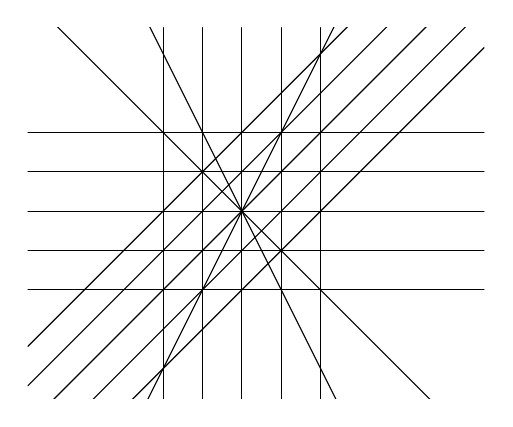
\begin{tikzpicture}[line cap=round,line join=round,>=triangle 45,x=.5cm,y=.5cm]
\clip(-5.44,-4.76) rectangle (6.16,4.66);
\draw [domain=-5.44:6.16] plot(\x,{(-0.0-1.0*\x)/-1.0});
\draw (0.0,-4.76) -- (0.0,4.66);
\draw [domain=-5.44:6.16] plot(\x,{(-0.0-0.0*\x)/1.0});
\draw [domain=-5.44:6.16] plot(\x,{-2.0*\x});
\draw [domain=-5.44:6.16] plot(\x,{(-0.0--2.0*\x)/1.0});
\draw [domain=-5.44:6.16] plot(\x,{(-0.0--1.0*\x)/-1.0});
\draw [domain=-5.44:6.16] plot(\x,{(-2.0-0.0*\x)/-1.0});
\draw [domain=-5.44:6.16] plot(\x,{(-1.0-0.0*\x)/-1.0});
\draw [domain=-5.44:6.16] plot(\x,{(--1.0--0.0*\x)/-1.0});
\draw [domain=-5.44:6.16] plot(\x,{(--2.0--0.0*\x)/-1.0});
\draw (-2.0,-4.76) -- (-2.0,4.66);
\draw (-1.0,-4.76) -- (-1.0,4.66);
\draw (1.0,-4.76) -- (1.0,4.66);
\draw (2.0,-4.76) -- (2.0,4.66);
\draw [domain=-5.44:6.16] plot(\x,{(--1.0--1.0*\x)/1.0});
\draw [domain=-5.44:6.16] plot(\x,{(--2.0--1.0*\x)/1.0});
\draw [domain=-5.44:6.16] plot(\x,{(-1.0--1.0*\x)/1.0});
\draw [domain=-5.44:6.16] plot(\x,{(-4.0--2.0*\x)/2.0});
\end{tikzpicture}
\caption{A configuration of 19 lines (the line at infinity, $z=0$, is not shown).}
\label{H19Fig}
\end{center}
\end{figure}

\begin{figure}[htbp]
\begin{center}
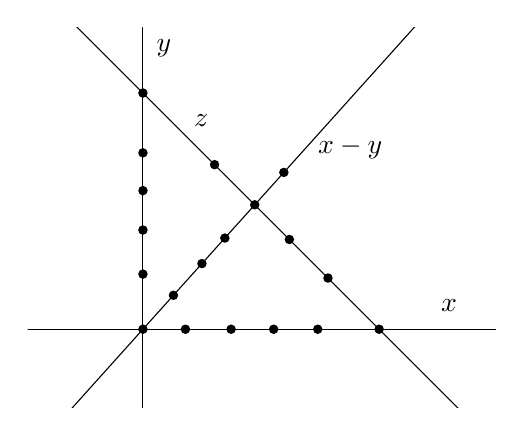
\begin{tikzpicture}[line cap=round,line join=round,>=triangle 45,x=1.0cm,y=1.0cm]
\clip(-1.463688897430969,-0.9982420398488032) rectangle (4.481599077455316,3.829741815619195);
\draw (0.0,-0.9982420398488032) -- (0.0,3.829741815619195);
\draw [domain=-1.463688897430969:4.481599077455316] plot(\x,{(--9.0-3.0*\x)/3.0});
\draw [domain=-1.463688897430969:4.481599077455316] plot(\x,{(-0.0-0.0*\x)/3.0});
\draw [domain=-1.463688897430969:4.481599077455316] plot(\x,{(-0.0--1.58*\x)/1.42});
\draw (3.6615593567813454,0.5) node[anchor=north west] {$x$};
\draw (0.5249074252034089,2.845694150810431) node[anchor=north west] {$z$};
\draw (0.05,3.8) node[anchor=north west] {$y$};
\draw (2.1,2.5586802485745417) node[anchor=north west] {$x-y$};
\begin{scriptsize}
\draw [fill=black] (0.0,0.0) circle (1.5pt);
\draw [fill=black] (0.0,3.0) circle (1.5pt);
\draw [fill=black] (3.0,0.0) circle (1.5pt);
\draw [fill=black] (0.0,0.7) circle (1.5pt);
\draw [fill=black] (0.0,1.26) circle (1.5pt);
\draw [fill=black] (0.0,1.76) circle (1.5pt);
\draw [fill=black] (0.0,2.24) circle (1.5pt);
\draw [fill=black] (1.42,1.58) circle (1.5pt);
\draw [fill=black] (0.91,2.09) circle (1.5pt);
\draw [fill=black] (1.86,1.140) circle (1.5pt);
\draw [fill=black] (2.35,0.65) circle (1.5pt);
\draw [fill=black] (0.38753589789044496,0.43120191455415724) circle (1.5pt);
\draw [fill=black] (0.7492696330437865,0.8336943804290022) circle (1.5pt);
\draw [fill=black] (1.0403935472433967,1.157620989186315) circle (1.5pt);
\draw [fill=black] (1.7896631802871834,1.9913153696153176) circle (1.5pt);
\draw [fill=black] (0.54,0.0) circle (1.5pt);
\draw [fill=black] (1.12,0.0) circle (1.5pt);
\draw [fill=black] (1.66,0.0) circle (1.5pt);
\draw [fill=black] (2.22,0.0) circle (1.5pt);
\end{scriptsize}
\end{tikzpicture}
\caption{A sketch of the points dual to the lines of the line configuration given in Figure \ref{H19Fig}.}
\label{dualH19Fig}
\end{center}
\end{figure}

\noindent It is not hard to verify that the first difference of the Hilbert function of $Z$ is $\Delta h_Z = (1,2,3,4,4,4,1)$, from which  we find that $t_Z=9$. Picking a random point $P$, Macaulay2 \cite{M2} finds that $[I_{Z+7P}]_8=0$. By upper semicontinuity,
this means $m_Z>7$. Thus we have $8\leq m_Z\leq t_Z=9$.
Using our results up to now, we cannot determine whether  $m_Z=8$ or $m_Z=9$.
 In Example \ref{H_19Finished}   we will show that $m_Z=8$,  so $Z$ has an unexpected curve of degree 9. 
\end{example}

\section{Further criteria} 
  \label{sec:criteria}

In this section we establish additional facts about the invariants that we introduced in the preceding sections, and about the property of being generally special.  We also discuss irreducibility of unexpected curves. 

Recall that, for a set of points $Z$ of ${ \ensuremath{\mathbb{P}}}^2$ and another point $P \notin Z$, the dimension of  $H^0((\mathcal I_{Z + m_Z P}(m_Z+1))$ is one or two (see Lemma \ref{lem:dim estimate}).  Extending Proposition \ref{uniqueUnexpCurveOfLeastDegree}, our first result describe which value occurs if $P$ is a general point. It also gives a numerical characterization of a generally special set of points. Notice that the definitions immediately imply that a finite set of points $Z$ is generally special if and only if $m_Z < u_Z$. We continue to use the assumption that $Z$  consists of at least two points. 

\begin{theorem} 
   \label{thm:dim is two}
Let $Z \subset { \ensuremath{\mathbb{P}}}^2$ be a finite set, and let $P \in { \ensuremath{\mathbb{P}}}^2$  be a general point. If the base  field $K$ is infinite, then one has: 
\begin{itemize}
\item[(a)] The following three conditions are equivalent: 
\begin{itemize}
\item[(i)] $m_Z > u_Z$. 

\item[(ii)] $\dim_K [I_{Z + m_Z P}]_{m_Z + 1} = 2$. 

\item[(iii)] $|Z| = 2 m_Z + 1$. 
\end{itemize}

Furthermore, any of these conditions implies $u_Z = m_Z - 1$. 

\item[(b)] $m_Z = u_Z$ if and only if $|Z| = 2 m_Z + 2$. 

\item[(c)] $m_Z <  u_Z$ if and only if $|Z| \ge  2 m_Z + 3$.  
\end{itemize}   
\end{theorem}

\begin{proof} Let $\ell$ be a general linear form in  $I_P$. As observed above, then   $(I_P^{m_Z}, \ell) = (\ell, f)$, where  $f \in I_P^{m_Z}$ is  a form of degree $m_Z$.  We denote by ${H_{\mathfrak m}}^i (M)$ the $i$-th local cohomology module of a graded $R$-module $M$ with support in ${\mathfrak m} = (x, y, z)$. 

By definition,  $m_Z = 0$ if and only if $Z$ is collinear. In this case, we get $u_Z = |Z| - 2$  by Corollary \ref{u_ZCor}. Moreover, $|Z| \ge 2$ by assumption,  Hence, we may assume $m_Z \ge 1$ for the remainder of the proof. 

First, we show (a). Assume $\dim_K [I_{Z + m_Z P}]_{m_Z + 1} = 2$. Then Sequence \eqref{eq:exact sequence} gives 
\[
m_Z = \dim_K [R/(I_{Z + m_Z P}, \ell)]_{m_Z + 1} = \dim_K [R/(\ell, f)]_{m_Z + 1}. 
\]
Since the saturation of $(I_{Z + m_Z P}, \ell)$ is $(I_P^{m_Z}, \ell) = (\ell, f)$, and the latter ideal has minimal generators whose degrees are at most $m_Z$, we conclude that 
\[
[(I_{Z + m_Z P}, \ell)]_{j} = [(\ell, f)]_j \quad \text{ whenever } j \ge m_Z + 1. 
\]
Furthermore, Lemma \ref{lem:initial degree} yields   $[I_{Z + m_Z P}]_{m_Z} = 0$ because $m_Z \le t_Z \le \frac{|Z| - 1}{2}$ by Corollary \ref{mz<tzCor}. It follows that 
\[
{H_{\mathfrak m}}^0 (R/(I_{Z + m_Z P}, \ell) \cong (\ell, f)/(I_{Z + m_Z P}, \ell) \cong K (-m_Z). 
\]
The sequence in local cohomology induced by Sequence \eqref{eq:exact sequence} begins 
\[
0 \to K (-m_Z) \to {H_{\mathfrak m}}^1 (R/I_{Z + (m_Z - 1) P}) (-1) \to {H_{\mathfrak m}}^1 (R/I_{Z + m_Z P}) \to {H_{\mathfrak m}}^1 (R/(\ell, f). 
\]

By Proposition \ref{uniqueUnexpCurveOfLeastDegree}, the assumption $\dim_K [I_{Z + m_Z P}]_{m_Z + 1} = 2$ implies  that $Z$ is not generally special, and hence $u_Z \le m_Z$. Assume $u_Z = m_Z$. By definition of $u_Z$, this means that $[{H_{\mathfrak m}}^1 (R/I_{Z + m_Z P})]_{m_Z + 1} = 0$ and $[{H_{\mathfrak m}}^1 (R/I_{Z + (m_Z -1) P})]_{m_Z} \neq 0$, which is a contradiction by the above exact sequence. It follows that $u_Z < m_Z$. 

Conversely, assume $u_Z < m_Z$. Consider the beginning of the long exact cohomology induced by Sequence \eqref{eq:exact sequence} 
\[
0 \to {H_{\mathfrak m}}^0 (R/(I_{Z + m_Z P}, \ell))  \to {H_{\mathfrak m}}^1 (R/I_{Z + (m_Z - 1) P}) (-1) \to {H_{\mathfrak m}}^1 (R/I_{Z + m_Z P}). 
\]
By Lemma \ref{cor:uZ implies} we know $[{H_{\mathfrak m}}^1 (R/I_{Z + (m_Z - 1) P})]_{m_Z} = 0$. It follows that 
\[
0 = [{H_{\mathfrak m}}^0 (R/(I_{Z + m_Z P}, \ell)]_{m_Z + 1}  \cong [(\ell, f)/(I_{Z + m_Z P}, \ell)]_{m_Z + 1}, 
\]
which implies $\dim_L [(I_{Z + m_Z P}, \ell)/(\ell) ]_{m_Z + 1} = 2$, and hence $\dim_L [I_{Z + m_Z P}]_{m_Z + 1} \ge 2$. Now Lemma \ref{lem:dim estimate} gives  equality. This concludes the proof that conditions (i) and (ii) are equivalent. 

By definition of $m_Z$, we have $h^0({ \ensuremath{\mathbb{P}}}^2,\mathcal I_{Z+(m_Z - 1) P}(m_Z)) = 0$. Applying Lemma \ref{lem:rewrite rhs}(b) with $j = m_Z-1$, we get 
\[
h^1({ \ensuremath{\mathbb{P}}}^2,\mathcal I_{Z+(m_Z - 1) P}(m_Z)) = |Z| - [2(m_Z -1) + 3]= |Z| - [2m_Z + 1].  
\]
It follows that $|Z| = 2 m_Z + 1$ if and only if $h^1({ \ensuremath{\mathbb{P}}}^2,\mathcal I_{Z+(m_Z - 1) P}(m_Z)) = 0$. By Lemma \ref{cor:uZ implies}, the latter condition is equivalent to $u_Z < m_Z$, which proves that conditions (i) and (iii) are equivalent. 

For (a), it remains to show that $u_Z = m_Z - 1$. This is clear if $m_Z = 1$. Let $m_Z \ge 2$. 
The definition of $m_Z$ also gives $h^0({ \ensuremath{\mathbb{P}}}^2,\mathcal I_{Z+(m_Z - 2) P}(m_Z -1)) = 0$. Applying Lemma \ref{lem:rewrite rhs}(b) with $j = m_Z -2$, we obtain
\[
h^1({ \ensuremath{\mathbb{P}}}^2,\mathcal I_{Z+(m_Z - 2) P}(m_Z -1)) = |Z| - [2(m_Z -2) + 3] = 2, 
\]
which proves $u_Z = m_Z -1$. Now the proof of (a) is complete. 

Second, we show (b). Assume $u_Z = m_Z$. Combining part (a) and Lemma \ref{lem:dim estimate}, this gives $\dim_K [I_{Z + m_Z P}]_{m_Z + 1} = 1$. Moreover, by definition of $u_Z$ we have ${H_{\mathfrak m}}^1 (R/I_{Z + m_Z P})]_{m_Z + 1} = 0$. Hence, applying Lemma \ref{lem:rewrite rhs}(b) with $j = m_Z$, we obtain $|Z| = 2 m_Z + 2$, as desired. 

Conversely, assume $|Z| = 2 m_Z + 2$. Then part (a) implies $u_Z \ge m_Z$. If $m_Z <  u_Z$, then Proposition \ref{uniqueUnexpCurveOfLeastDegree}
 shows  $|Z| \ge  2 m_Z + 3$. It follows that we must have $u_Z = m_Z$, which completes the proof of (b). 

Part (c) follows from (a) and (b). 
\end{proof} 

Combining this with earlier results, we see that the multiplicity index and the speciality index are closely related. 

\begin{corollary}
   \label{cor:uZ}
If $Z \subset \mathbb P^2$ is any finite set of points, then $m_Z + u_Z = |Z| - 2$.    
\end{corollary}

\begin{proof}
If $2 m_Z +2 \ge |Z|$, then the claim follows from Theorem \ref{thm:dim is two}(a), (b). Thus, it remains to consider the case, where $2 m_Z + 3 \le |Z|$, that is, $Z$ is generally special. 
By Proposition \ref{uniqueUnexpCurveOfLeastDegree}, then the irreducible components of $C_Z$ consist of an irreducible curve $B_Z$ of 
some degree $t+1$ with multiplicity $t$ at $P$ and containing exactly $ |Z|-r$ points of $Z$, where  $r = m_Z - t$, 
and $r$ lines $L_i$ which go through $P$ and the $r$ points of $Z$ not on $B_Z$.  
We denote by $E$ the sum of the exceptional curves of the blowings up of the points 
of $Z$, by $E_P$ the blow up of $P$ and by $H$ the pullback of a line.
Let $C_Z^*$ be the proper transform of $C_Z$, $B_Z^*$ the proper transform of $B_Z$ 
and $L_i^*$ the proper transforms of the $L_i$. Setting $j = m_Z + s$, we have  
\[
\begin{array}{rcl}
h^1(\mathcal I_{Z+jP}(j+1)) & = & h^1(\mathcal I_{Z+(m_Z+s) P}(m_Z+s+1)) \\
& = & h^1 (\mathcal O_X (m_Z+s+1)H - E - (m_Z+s)E_P ) \\
& = & h^1(\mathcal O_X(C_Z^* + s(H-E_P))),
\end{array}
\]
so 
$u_Z$ is the least value of $s+m_Z$ such that these are 0. Since $Z$ is generally special we know that $u_Z > m_Z$, and thus $s > 0$.  Note that 
$\mathcal O_X(C_Z^*+s(H-E_P))=\mathcal O_X(B_Z^*+\sum_iL_i^*+s(H-E_P))$. Thus from the  standard short exact sheaf sequence 
\[
0 \to \mathcal O_X \to \mathcal O_X(B_Z^*) \to \mathcal O_{B_Z^*}(B_Z^* ) \to 0,
\]
we have
\[
0 \to \mathcal O_X(\sum_iL_i^*+s(H-E_P))\to \mathcal O_X(C_Z^*+s(H-E_P))\to \mathcal O_{B_Z^*}(C_Z^*+s(H-E_P))\to0.
\]
It is easy to see that $h^1$ of the leftmost term is 0 (note that the curves $L_i^*$ and $H-E_P$ are disjoint smooth rational curves of self-intersection
$-1$ or 0), so the $h^1$ of the middle term is at most equal to the $h^1$ of the rightmost term.
But $B_Z^*$ is smooth and rational, so $h^1$ here is 0 if and only if $(B_Z^*)\cdot (C_Z^*+s(H-E_P))\geq -1$.
Since $(B_Z^*)\cdot (C_Z^*+s(H-E_P))=(t+1)(m_Z+1)-tm_Z-(|Z|-r)+s=m_Z+t+1+r+s-|Z|=2m_Z+1+s-|Z|$,
we see being greater than or equal to $-1$ is equivalent to $s+m_Z\geq |Z|-m_Z-2$, hence $u_Z=|Z|-m_Z-2$.
\end{proof}

We know that  the existence of an unexpected curve to a set $Z$ implies that  $Z$ is generally special (see Lemma \ref{UnexpImpliesGenSpec}). The following result shows that the converse is not necessarily true. 

\begin{proposition}
   \label{prop:gen special not sufficient} 
Let  $Z \subset \mathbb P^2$ be a set of $d$ points such that there is a line $L$ that contains precisely $t \ge \frac{d+2}{2}$ of the points of  $Z$. Then one has: 
\begin{itemize}
\item[(a)] $m_Z = d - t$ and $u_Z = t-2$. 

\item[(b)] $Z$ does not admit an unexpected curve. 

\item[(c)] If $t \ge \frac{d+3}{2}$, then $Z$ is generally special. 
\end{itemize}   
\end{proposition}

\begin{proof}
Let $P$ be a general point, and set $m=d-t$. Note that $t\ge  \frac{d+2}{2}$ implies $t\geq m+2$. Thus, if  $j\le m$, then $L$ is a fixed component
of the linear systems of curves corresponding to both $[I_Z\cap I_P^j]_{j+1}$ and $[I_Z]_{j+1}$. It follows that  
 $\dim_K [I_Z\cap I_P^j]_{j+1}=\dim_K[I_Y\cap I_P^j]_j$ and $\dim_K[I_Z]_{j+1}=\dim_K[I_Y]_j$,
where $Y$ consists of the $m$ points of $Z$ not on $L$. By Lemma \ref{lem:initial degree},
$\dim_K[I_Y\cap I_P^m]_m=1$ and $\dim_K[I_Y\cap I_P^{m-1}]_{m-1}=0$.
Thus $\dim_K[I_Z\cap I_P^m]_{m+1} = 1$ but $\dim_K [I_Z\cap I_P^{m-1}]_m=0$, which gives $m_Z = m = d-t$, and so $u_Z = t-2$ by Corollary \ref{cor:uZ}, proving (a).  

Using Lemma \ref{lem:initial degree} again, we get 
$1=\dim_K [I_Z\cap I_P^m]_{m+1}=\dim_K [I_Y\cap I_P^m]_m=\dim_K [I_Y]_m-\binom{m+1}{2}=\dim_K [I_Z]_{m+1}-\binom{m+1}{2}$, and 
so $t_Z\leq m=m_Z\leq t_Z$. 
But now we have $m_Z = t_Z$, and so by Theorem \ref{u_ZTheorem}, $Z$ does not admit an unexpected curve, proving (b).

Finally (c) follows because $|Z| \ge \frac{d+3}{2}$ if and only if $d- t < t-2$, which by (a) is equivalent to  $Z$ being generally special. 
\end{proof} 

We now show that adding an irreducibility hypothesis forces the existence of an unexpected curve. 

\begin{corollary} 
   \label{cor:irr forces unexpected}
Let  $Z \subset \mathbb P^2$ be a generally special set of points such that  $[I_{Z+m_ZP}]_{m_Z+1}$ contains an irreducible form and $m_Z \ge 1$. Then $Z$ has an unexpected curve.
\end{corollary}

\begin{proof}
If $h_Z(t_Z) = |Z|$ then by Corollary \ref{u_ZCorB} we obtain that $Z$ has an unexpected curve. (We  did not need irreducibility.) 
Thus, it remains to rule out  that   $h_Z (t_Z) < |Z|$. Indeed, if $h_Z (t_Z) < |Z|$, then Theorem  \ref{thm:tZ = dZ} gives $m_Z = t_Z$.
By Proposition \ref{prop:small tZ}, there are two cases.  

\begin{itemize}

\item[-] In case (b)(i) we have that $Z$ is the complete intersection of a conic and a curve of degree $t_Z+1$, so $|Z| = 2t_Z+2$. Hence $|Z| = 2m_Z+2 < 2m_Z+3$. Contradiction. (Again we did not use irreducibility.)

\medskip

\item[-] In case (b)(ii), there is a line through $|Z|-t_Z \geq t_Z+2$ of the points, i.e. through $|Z| - m_Z \geq m_Z+2$ of the points. 
Thus this line is a component of any curve of degree $m_Z+1$ containing $Z + m_ZP$.
Since $m_Z>0$ and 
$h^0(\mathcal I_{Z+m_ZP}(m_Z+1))=1$ by Theorem \ref{thm:tZ = dZ}, 
we see that  there is no irreducible form
in $[I_{Z+m_ZP}]_{m_Z+1}$, contrary to assumption. 
\end{itemize} 
\end{proof}

We summarize some of our results by giving an extension of our criterion for unexpected curves, Theorem \ref{u_ZTheorem}.

\begin{theorem} \label{criterion}
The following conditions are equivalent for a reduced finite subscheme  $Z \subset \mathbb P^2$.

\begin{itemize}
\item[(a)] $Z$ has an unexpected curve;

\item[(b)] $m_Z < t_Z$;

\item[(c)] $m_Z < t_Z = \left \lfloor \frac{|Z| -1}{2} \right \rfloor$;

\item[(d)] $Z$ is generally special and $h_Z(t_Z) = |Z|$;

\item[(e)] $h_Z (t_Z) = |Z| \geq 2m_Z +3$.

\end{itemize}

\end{theorem}

\begin{proof}
The equivalence of (a) and (b) is Theorem \ref{u_ZTheorem}. 

By Theorem \ref{thm:tZ = dZ}, $m_Z < t_Z$ implies $h_Z (t_Z) = |Z|$, which is equivalent to $ t_Z = \left \lfloor \frac{|Z| -1}{2} \right \rfloor$ (see Corollary \ref{mz<tzCor}). This proves the equivalence of (b) and (c). 

Lemma \ref{UnexpImpliesGenSpec} shows that (a) implies (d).  The fact that (c) implies (a) is Corollary \ref{u_ZCorB}. The equivalence of (d) and (e) comes from Theorem \ref{thm:dim is two}.
\end{proof}

As a consequence, we get a first answer to Problem \ref{prob:intro} in the case, where $Z$ is reduced and $r=1$. 

\begin{proposition}
   \label{prop:intro}
Given a finite set of points $Z$  and a general point $P$. Then the subscheme $X = m P$ fails to impose the expected number of conditions on  $V = [I_Z]_{m+1}$ if and only if 
\begin{itemize}
\item[(i)]  $h^0 ({\mathcal{I}}_{Z + m P} (m+1)) \cdot h^1 ({\mathcal{I}}_{Z + m P} (m+1)) \neq 0$; \quad and 

\item[(ii)] $h^1 ({\mathcal{I}}_{Z} (t_Z)) = 0$. 
\end{itemize} 
\end{proposition}

\begin{proof}
Note that $h^0 ({\mathcal{I}}_{Z + mZ} (m+1)) \neq 0$ is equivalent to $m_Z \le m$. Furthermore, using Lemma \ref{cor:uZ implies}, one sees that  $h^1 ({\mathcal{I}}_{Z + mZ} (m+1)) \neq 0$ is equivalent to $m+1 \le u_Z$. Hence, Condition (i) of the statement means $m_Z < m \le u_Z$, which in particular shows that $Z$ is generally special. Condition (ii) is equivalent to $h_Z (t_Z) = |Z|$. We conclude by using  Theorems \ref{criterion} and \ref{u_ZTheorem}. 
\end{proof}

\begin{remark}
   \label{rem:question}
Fix an integer $m \ge 1$, and let $Z \subset { \ensuremath{\mathbb{P}}}^2$ be a finite set of points. If $P$ is a general point of ${ \ensuremath{\mathbb{P}}}^2$, we have seen in Lemma \ref{lem:initial degree} that $mP$ imposes the expected number of conditions on $[I_Z]_j$ if $j \le m$, whereas this may fail if $j = m+1$. We wonder if this degree is the only degree where such failure can occur. In other words, we pose the following 
\smallskip 

\noindent
{\bf Question:} If $mP$ does not impose the expected number of conditions on $[I_Z]_j$ for some integer $j$, is it then true that $j$ must equal $m+1$?
\end{remark} 

We now consider the change of the multiplicity index if one adds a point to a given set of points. 

\begin{lemma} \label{lem:change of index}
Let $P_1,\ldots,P_s,P,Q$ be distinct points of ${ \ensuremath{\mathbb{P}}}^2$,  with $P$ a general point, and let $Z=P_1+\cdots+P_s$.
Then $m_{Z+Q,P}=m_Z$ if either $\dim_K [I_Z\cap I_P^{m_Z}]_{m_Z+1}>1$ or
$Q$ is a base point of $[I_Z\cap I_P^{m_Z}]_{m_Z+1}$. Otherwise, 
$m_{Z+Q,P}=m_Z+1$.
\end{lemma}

\begin{proof}
For each integer $j \ge 0$, one has $I_{Z+Q} \cap I_P^j \subset I_Z \cap I_P^j$,
hence $m_{Z+Q,P}\geq m_Z$. If $Q$ is a base point of $[I_Z\cap I_P^{m_Z}]_{m_Z+1}$,
then $\dim[I_{Z+Q}\cap I_P^{m_Z}]_{m_Z+1}= \dim_K [I_Z\cap I_P^{m_Z}]_{m_Z+1}\geq 1$,
so $m_{Z+Q,P}=m_Z$. If $\dim_K [I_Z\cap I_P^{m_Z}]_{m_Z+1}>1$, then, since
$\dim_K [I_{Z+Q}\cap I_P^{m_Z}]_{m_Z+1}$ drops by at most 1, we have 
$\dim[I_{Z+Q}\cap I_P^{m_Z}]_{m_Z+1}\geq 1$, and again $m_{Z+Q,P}=m_Z$.
If $Q$ is not a base point of $[I_Z\cap I_P^{m_Z}]_{m_Z+1}$, then the dimension
drops exactly one, so if also $\dim_K [I_Z\cap I_P^{m_Z}]_{m_Z+1}=1$
we get $\dim[I_{Z+Q}\cap I_P^{m_Z}]_{m_Z+1}= 0$, hence $m_{Z+Q,P}\geq m_Z+1$.
But let $f \neq 0$ be a form of degree $m_Z + 1$ 
in $I_Z \cap I_P^{m_Z}$. Let $\ell$ be a linear form that defines the line through $P$ and $Q$. Then 
$\ell f \neq 0$ is in $[I_{Z+Q} \cap I_P^{m_Z+1}]_{m_Z+2}$, which shows $m_{Z+Q, P} \le m_Z+1$. 
\end{proof} 

Thus, given $m_Z$, there are only two possible values of $m_{Z+Q}$. 
When the number points of $Z$ is odd and  $m_Z$ is as large as possible, we can say which of these values occurs for an arbitrary point $Q$.

\begin{proposition} \label{prop:change of mZ, max mZ}
Let $Z$ be a finite reduced subscheme of ${ \ensuremath{\mathbb{P}}}^2$.
If $m_Z = \frac{|Z| - 1}{2}$, then $m_{Z + Q} = m_Z$ for any point $Q$ not in $Z$.
\end{proposition} 

\begin{proof}
By Corollary \ref{mz<tzCor} we get $m_Z=t_Z = \frac{|Z|-1}{2}$.  Thus,  Lemma \ref{lem:rewrite rhs}(b) implies 
\[
h^0((\mathcal I_Z \otimes \mathcal I_P^{m_Z})(m_Z+1)) \ge 
2m_Z + 3 - |Z| =2. 
\]
Now the result follows by Lemma \ref{lem:change of index}.
\end{proof}

If  $m_Z < \frac{|Z|-1}{2}$ and $Q$ is a \emph{general} point,  we now find the value of $m_{Z+Q}$.

\begin{proposition} \label{conj:change of dZ}
Let $Z$ be a finite reduced subscheme of ${ \ensuremath{\mathbb{P}}}^2$ and let $Q$ be a general point.
If $m_{Z} < \frac{|Z| - 1}{2}$, then $m_{Z + Q} = m_Z + 1$.
\end{proposition}

\begin{proof}
If $m_{Z} < \frac{|Z| - 1}{2}$, then Theorem \ref{thm:dim is two}(a) gives $\dim_K [I_{Z + m_Z P}]_{m_Z + 1} = 1$. Hence the result follows from Lemma \ref{lem:change of index}. 
\end{proof}

 We will  observe on more than one occasion below that it is of interest to know when $Z$ admits an {\em irreducible} unexpected curve of minimal degree $m_Z+1$. Furthermore,  Corollary \ref{cor:irr forces unexpected} shows that  this is related to the  existence of an irreducible form in $[I_{Z+m_ZP}]_{m_Z+1}$. 
 These facts motivate the next result. 

\begin{corollary} 
       \label{irred curve least deg}
Assume that $Z$ is a finite set of points in $\mathbb P^2$ such that $2 m_Z + 2 \le |Z|$. Let $P \in { \ensuremath{\mathbb{P}}}^2$ be a general point.   Then $[I_{Z+m_ZP}]_{m_Z+1}$ contains an  irreducible form  if and only if $m_{Z - Q} = m_Z$ for each point $Q \in Z$.
\end{corollary}

\begin{proof}
By Theorem \ref{thm:dim is two},  there is a unique curve $C$ of degree $m_Z+1$ vanishing at $Z$ and to order $m_Z$  at the general point $P$.   

If $m_{Z-Q} = m_Z -1$ (the only other possibility), let $F$ be a form in $[I_{Z-Q}]_{m_Z}$ vanishing to order $m_Z -1$ at  $P$; by abuse of notation we will also denote by $F$ the curve that it defines. Then if $\ell$ is the line joining $Q$ to $P$, $\ell  F$ must equal $C$, hence $C$ is not irreducible.

Conversely, assume that $m_{Z-Q} = m_Z$ for all $Q \in Z$. By Proposition \ref{uniqueUnexpCurveOfLeastDegree} (iv), if $C$ is not irreducible then there is at least one component of $C$ consisting of a line joining $P$ and a point $Q \in Z$. Removing this point and this line shows that $m_{Z-Q} = m_Z -1$, giving a contradiction.
\end{proof}

We will apply this irreducibility criterion to give examples of irreducible unexpected  curves in the following section  when we have further methods to compute multiplicity indices. 
We conclude this section by showing that an unexpected curve cannot be completely decomposable, that is, be a union of lines. But first we need a lemma. 

\begin{lemma}
   \label{LinesLemma}
Let $Y$ be a set of $m$ points in ${ \ensuremath{\mathbb{P}}}^2$, and let $P \in { \ensuremath{\mathbb{P}}}^2$ be a point that is not on any line through two of the points of $Y$.    Let $X \subset { \ensuremath{\mathbb{P}}}^2$ be a set of $u \ge m+2$ points on a line $L$ such that  none of the points in $Y$ nor $P$ is on $L$. Set $Z = Y \cup X$. Then for $ m+1 \leq  j+1<u$ we have $\dim_K [I_{Z+mP}]_{j+1}=\dim_K [I_{Y+mP}]_j=\binom{j+2}{2}-\binom{m+1}{2}-m$ and
$\dim_K [I_Z]_{j+1}=\dim_K [I_Y]_j=\binom{j+2}{2}-m$,
while for $j+1\geq u$ we have $\dim_K [I_{Z+mP}]_{j+1}=\binom{j+3}{2}-\binom{m+1}{2}-m-u=\dim_K [I_Z]_{j+1}-\binom{m+1}{2}$.
\end{lemma} 

\begin{proof}
Let $\ell$ be a linear form defining $L$. Then there are exact sequences
\[
0 \to (R/I_Y) (-1) \to R/I_Z \to R/(I_Z, \ell) \to 0
\]
and 
\[
0 \to (R/I_{Y + mP}) (-1) \to R/I_{Z+m P} \to R/(I_{Z+m P}, \ell) \to 0. 
\]
Since the saturation of both of  $(I_Z, \ell)$ and $(I_{Z+j P}, \ell)$ is generated by $\ell$ and a form of degree $u$, we get $\dim_K [I_{Z+mP}]_{j+1}=\dim_K [I_{Y+mP}]_j$ and $\dim_K [I_Z]_{j+1}=\dim_K [I_Y]_j$ if $j+1 < u$. Combining Lemmas \ref{lem:uZ estimate} and \ref{cor:uZ implies}, we get $H^1(\mathcal I_{Y+mP}(j+1))=0$ if $j \ge m$. Moreover, we have $H^1(\mathcal I_Y(j)) = 0$ if $j \ge m$. This gives  $H^1(\mathcal I_{Z+mP}(j+1))=0 =  H^1(\mathcal I_Z(j))$ if $j+1\ge u$, 
Now the formulas for the dimensions follow. 
\end{proof}

\begin{corollary}\label{CurveComponentsCor}
Let $Z$ be a reduced 0-dimensional subscheme of ${ \ensuremath{\mathbb{P}}}^2$, and let $P$ be a general point.
If $Z$ has an unexpected curve, then the unique unexpected curve of degree $m_Z+1$ has a  unique component of degree more than 1. 
\end{corollary}

\begin{proof}
Lemma \ref{UnexpImpliesGenSpec} gives that $Z$ is generally special. Hence, 
by Proposition \ref{uniqueUnexpCurveOfLeastDegree} we know that there is a unique curve $C_Z$ of degree $m_Z + 1$ vanishing at $Z$ and to order $m_Z$ at $P$ and that $C_Z$ has a unique component $B_Z$ of degree $t+1$ vanishing to order $t \ge 0$ at $P$. We have to  that $t>0$ if $Z$ has unexpected curves.  

Assume, on the contrary, that $t=0$.
Note that then $C_Z$ has $m_Z$ lines through $P$, and these also go through $m_Z$ points of $Z$;
let $Y$ denote the scheme of these $m_Z$ points of $Z$.
The only other component of $C_Z$ is $B_Z$, also a line, and it contains the other $u=|Z|-m_Z$ points of $Z$.
From Proposition \ref{uniqueUnexpCurveOfLeastDegree} we have
$(m_Z+1)^2-m_Z^2-|Z|\leq -2$, hence $m_Z+3\leq |Z| -m_Z=u$. I.e., at least
$m_Z+3$ of the points of $Z$ lie on the line $C'_Z$.
Applying Lemma \ref{LinesLemma} with $m=m_Z$ and $L=C'_Z$ shows that
$\dim_K [I_{Z+mP}]_{j+1}=\dim_K [I_{Y+mP}]_j=\dim_K [I_Y]_j-\binom{j+2}{2}=\dim_K [I_Z]_{j+1}-\binom{j+2}{2}$
for $j+1<u$ and
$\dim_K [I_{Z+mP}]_{j+1}=\dim_K [I_Z]_{j+1}-\binom{m+1}{2}$ when $j+1\geq u$.
Thus $Z$ has no unexpected curves if $t=1$.
\end{proof}

\section{Line arrangements and multiplicity indices}  \label{arrangement section}

We now assume that the base field $K$ has characteristic zero. The results that we obtained in the previous sections about  sets of points and the unexpected curves associated to them have a beautiful application to the line arrangements dual to those points, advancing the known theory about this connection.

Let ${\mathcal{A}}$ be a line arrangement in ${ \ensuremath{\mathbb{P}}}^2$; i.e. ${\mathcal{A}}$ is a set of lines defined by a reduced product, $f$,
of linear forms. The Jacobian ideal of $f$, $J = \operatorname{Jac}(f) = (f_x, f_y, f_z)$, fits into an exact sequence of graded $R$-modules 
\[
0 \rightarrow F_2 \rightarrow F_1\rightarrow R(-(\deg f -1))^3 \rightarrow J \rightarrow 0, 
\]
where $F_1$ and $F_2$ are finitely generated free $R$-modules.  Let $D_0$ be the cokernel of $F_2 \rightarrow F_1$; the sheafification of $D_0$ is called the {\em syzygy bundle}. 
Sheafifying and twisting by $\deg(f)-1$ gives an exact sheaf sequence
\[
0 \rightarrow \mathcal D \rightarrow \mathcal O_{{ \ensuremath{\mathbb{P}}}^2}^3 \rightarrow \mathcal J(\deg(f)-1) \rightarrow 0
\]
where $\mathcal D$ is the sheafification of  $D(f) = D_0(\deg f-1)$, called the {\em derivation bundle} of ${\mathcal{A}} = {\mathcal{A}} (f)$.
Indeed,  $\mathcal D$ is locally free  of rank two. 
By Grothendieck's theorem, the restriction of $\mathcal D$ to a general line has the form 
$\mathcal O_{\mathbb P^1}(-a) \oplus \mathcal O_{\mathbb P^1}(-b)$ for some integers $a\leq b$.
We refer to $(a,b)$ as the \emph{splitting type} of ${\mathcal{A}}$. Note that $a + b = \deg f  - 1$. 

Moreover, one says that the arrangement  ${\mathcal{A}}$ is \emph{free} if the module $D_0$ is a free $R$-module, which is true if and only if the Jacobian ideal $ J$ is saturated. In this case, ${\mathcal{A}}$ having splitting type $(a, b)$ is equivalent to $D_0 (\deg f - 1) \cong R(-a) \oplus R(-b)$, and one also says that $\mathcal A$ is \emph{free with exponents $(a,b)$}. In particular, if $ J$ has only two minimal generators, then  the arrangement ${\mathcal{A}}$ is free with exponents $(0, \deg f -1)$.  It is not hard to see that this happens if and only if every line in ${\mathcal{A}}$ passes through a single point $P$. 

\begin{remark} \label{stefan}
A line arrangement $\mathcal A$ in $\mathbb P^2$ is {\em supersolvable} if it has a so-called {\em modular point}, i.e. a point $P$ with the property that if $\ell_1, \ell_2 \in \mathcal A$ and if $Q$ is the intersection of $\ell_1$ and $\ell_2$ then the line joining $P$ and $Q$ is a line of $\mathcal A$. A standard fact is that if $\mathcal A$ is a supersolvable line arrangement consisting of $d$ lines, $m$ of which pass through the  modular point $P$, then $\mathcal A$ is free, and the splitting type is $(m-1,d-m)$. We are grateful to S. Toh\^{a}neanu for pointing out that the computation of the splitting type is a simple application of the addition-deletion theorem (Theorem \ref{add-del} below) using induction on $d$, with  the base case being the case that all lines pass through a single point, mentioned above. 
\end{remark}

The connection to the previous section is given by the following result. 

\begin{theorem}[Faenzi and Vall\`es] 
    \label{FVstrong}
Let ${\mathcal A} (f)$ be a line arrangement in $\mathbb P^{2\vee}$ 
  with splitting type  $(a, b)$, where $a \le b$. Let 
$Z \subset { \ensuremath{\mathbb{P}}}^2$ be the set of points dual to the lines in  $\mathcal A (f)$.   Then $m_Z = a$. That is, for a general 
point $P \in \mathbb P^2$ , 
\[
h^0(\mathcal I_Z \otimes \mathcal I_P^a)(a+1) \neq 0 \ \ \hbox{ and } \ \ 
h^0(\mathcal I_Z \otimes \mathcal I_P^{a-1})(a) = 0.
\]
\end{theorem} 

\begin {proof}
This follows from \cite[Theorem 4.3]{FV2}. 
\end{proof} 

Applying Corollary \ref{cor:uZ}, there is also an interpretation of $b$. 

\begin{corollary}
   \label{cor:precise interprete b}
If a line arrangement $\mathcal A(f)$ has splitting type $(a, b)$ and $Z$ is the dual set of points, then $b = u_Z + 1$.    That is, for a general 
point $P \in \mathbb P^2$, 
\[
h^1((\mathcal I_Z \otimes \mathcal I_P^{b-1})(b)) = 0 \ \ \hbox{ and } \ \ 
h^1((\mathcal I_Z \otimes \mathcal I_P^{b-2})(b-1)) \neq 0.
\]
\end{corollary}

\begin{proof}
Combine Theorem \ref{FVstrong} and Corollary \ref{cor:uZ}. 
\end{proof} 

Using the above interpretations of the splitting type, we record some consequences of the results in the previous sections for line arrangements. 

\begin{proposition} \label{gen spec splitting type}
Let $\mathcal A$ be an arrangement of  lines with splitting type of $\mathcal A$ is $(a,b)$, with $a  \leq b$. Let $Z$ be the set of points dual to the lines of $\mathcal A$. Then one has: 
\begin{itemize}

\item[(a)] $Z$ is generally special if and only if $b-a \geq 2$. 

\item[(b)]   If $b-a \geq 2$, $a \ge 2$,  and $[I_{Z+m_ZP}]_{m_Z+1}$ contains an irreducible form then $Z$ admits an unexpected curve. 

\item[(d)] If $b-a \geq 2$ but there is no irreducible form in $[I_{Z+m_ZP}]_{m_Z+1}$, then $Z$ does not necessarily have an unexpected curve, regardless of the value of $b-a$.

\end{itemize}
\end{proposition}

\begin{proof}
Part (a) follows from Theorem \ref{thm:dim is two}. Part (b) is a consequence of Corollary \ref{cor:irr forces unexpected},  while (c) follows from Proposition \ref{prop:gen special not sufficient}.
\end{proof}

\begin{remark}
The preceding proposition shows that the condition $b-a \geq 2$  is not enough to guarantee that $Z$ has an unexpected curve. We also note that 
the existence of an unexpected curve does not depend on the freeness of the syzygy bundle, as demonstrated by Proposition \ref{FermatProp} 
and Example \ref{H_19Finished} below, which are concerned with free and non-free arrangements, respectively.
\end{remark} 

The result mentioned in the introduction follows easily now. 

\begin{proof}[Proof of Theorem \ref{thm:intro}]
Combine Theorems \ref{u_ZTheorem}, \ref{FVstrong}, and Corollary \ref{cor:precise interprete b}. 
\end{proof}

For another consequence of our results on points we need some preparation. We begin by recalling 
a very special case of a construction that was introduced in \cite{LR} and that has been 
generalized quite extensively in the decades that followed. We present only the elementary 
version that we will use here. See for instance \cite{BM4}.

\begin{lemma} \label{BDL}
Let $I_X$ be the saturated ideal of a scheme $X$ in $\mathbb P^2$. Let $f \in I_X$ 
be a homogeneous polynomial. Let $\ell$ be a linear form such that $\ell$ does not 
vanish on any component of $X$. Let $Y$ be the complete intersection scheme 
with homogeneous ideal $(\ell,f)$. Then $\ell \cdot I_X + (f)$ is the saturated ideal of the scheme $X \cup Y$.
\end{lemma} 

\begin{lemma}
    \label{lem:non-free} 
Let ${\mathcal{A}} (f)$ be a line arrangement of $d \ge 3$ lines, and let $\ell$ be a linear form defining a line that meets ${\mathcal{A}} (f)$ in $d$ distinct points. Then the line arrangement ${\mathcal{A}} (f \ell)$ is free if and only if the $d$ lines of ${\mathcal{A}} (f)$ all meet in one point. 
\end{lemma}

\begin{proof}
Let $X \subset { \ensuremath{\mathbb{P}}}^2$ be the zero-dimensional subscheme defined by the Jacobian ideal of $f$. By assumption, the Jacobian ideal of $f \ell$ defines the subscheme $X \cup Y$, where $Y$ is the complete intersection defined by the ideal $\ell, f)$. By Lemma \ref{BDL}, the homogeneous ideal of $X \cup Y$ is $\ell I_X + (f)$. Since $f$ is not a minimal generator of $I_X$,  the product of $\ell$ and the minimal generators of $I_X$ together with $f$ form a minimal generating set of  $\ell I_X + (f)$ (see \cite[Corollary 4.5]{MN}). Hence this ideal has one minimal generator more than $I_X$. 

Now, if ${\mathcal{A}} (f \ell)$ is free, then $\operatorname{Jac} (f \ell) = \ell I_X + (f)$ has at most three minimal generators. It follows that in this case the ideal $I_X$ has two minimal generators of degree $d-1$. Since $I_X$ is the saturation of $\operatorname{Jac} (f)$, we get $I_X = \operatorname{Jac} (f)$. As observed above, this means that the lines of ${\mathcal{A}} (f)$ pass though a single point, as desired.  

Conversely, if $\operatorname{Jac} (f)$ is generated by two forms of degree $d-1$, then the saturation of $\operatorname{Jac} (f \ell)$ has three minimal generators of degree $d$. It follows that $\operatorname{Jac} (f) = \ell I_X + (f)$ is saturated, that is, ${\mathcal{A}} (f \ell)$ is free, which completes the argument. 
\end{proof}

\begin{proposition} \label{prop:many concurrent lines} 

Let $\mathcal A$ be an arrangement of $d$ lines in $\mathbb P^2$.  Assume that there is a point $Q$ through which there pass $t$ lines of 
$\mathcal A$, with $\frac{d+2}{2} \leq t$, and assume that none of the other lines pass through $Q$. Let $Z$ be the set of points dual to $\mathcal A$.
Then:
\begin{itemize}

\item[(a)] $\mathcal A$ has splitting type $(d-t,t-1)$;

\item[(b)]  $m_Z = d-t$;

\item[(c)] $Z$ does not admit an unexpected curve;

\item[(d)] If $\frac{d+3}{2} \leq t$ then $Z$ is generally special;

\item[(e)] If $t \leq d-2$ and if, at all  points of $\mathbb P^2$ other than $Q$, at most two lines of $\mathcal A$ pass, then $\mathcal A$ is not free.

\end{itemize}
\end{proposition}

\begin{proof}
Parts (b) - (d) are a consequence of Proposition \ref{prop:gen special not sufficient}.  Theorem \ref{FVstrong} and (b)  give (a). 

We now prove (e). 
Notice first that the assumptions force $d \geq 6$. They also force the number of lines {\em not} through 
$Q$, i.e. $d-t$, to satisfy $2 \leq d-t \leq \frac{d-2}{2}$.
Let $\mathcal B \subset \mathcal A$ be the set of lines 
through $Q$. By assumption, ${\mathcal{A}}$ is obtained from ${\mathcal{B}}$ by adding successively lines such that each line meets each of the previous lines in distinct points. Since we have to add at least two such lines to ${\mathcal{B}}$, Lemma \ref{lem:non-free} shows that ${\mathcal{A}}$ is not free. 
\end{proof} 

We now consider the change of the splitting type if one adds a line to an arrangement. 

\begin{proposition} 
  \label{prop:change of splitting type}
Let ${\mathcal A}(f) \subset { \ensuremath{\mathbb{P}}}^2$ be an arrangement of $d$ lines with splitting type $(a, b)$, where $a \le b$.  Let $\ell \in R$ be a linear form. Then one has: 
\begin{itemize}
\item[(a)] The splitting type of ${\mathcal{A}} (\ell f)$ is $(a+1, b)$ or $(a, b+1)$. 

\item[(b)] If $\ell$ is a general linear form, then 
\begin{itemize}
\item  ${\mathcal A} (\ell  f)$ has splitting type $(a, a+1)$ if  $(a, b) = (\frac{d-1}{2}, \frac{d-1}{2})$; \; and 

\item  ${\mathcal A} (\ell f)$ has splitting type $(a + 1, b)$ if  $a < \frac{d-1}{2} < b$. 
\end{itemize} 
\end{itemize} 
\end{proposition}

\begin{proof}
This follows by combining Theorem \ref{FVstrong} and Lemma \ref{lem:change of index} as well as Propositions \ref{prop:change of mZ, max mZ} and \ref{conj:change of dZ}.  \end{proof}

It is worth pointing out  that the splitting type  of a line arrangement can in principle be computed using computer algebra software. 

\begin{remark}
   \label{rem:compute split type}
Suppose that we are given the form $f$ defining a line configuration $\mathcal A(f)$ and we wish to compute $m_Z$ for the union of points, $Z$,  dual to the lines. This can arise, for example, if we know the coordinates for the individual points; it can also arise if we are given only the ideal of the points, since $f$ can be computed symbolically  from the ideal \cite{MP}.
Say $\deg f = d$. Let $J$ be the Jacobian ideal $(f_x, f_y,f_z)$. 
If $\mathcal A(f)$ is free, we have seen above how to compute the splitting type from a   minimal free resolution of $J$.  

Now assume that $\mathcal A(f)$ is not free. Let $\ell$ be a general linear form. Compute a minimal free resolution of $\bar J = \frac{J+(\ell)}{(\ell)}$ over $\bar R$. It has the form 
\[
0 \rightarrow \mathbb F_2 \rightarrow \bar{R}^3 (-d+1) \rightarrow \bar J \rightarrow 0, 
\]
where $\mathbb F_2$ (necessarily) has rank 2. If it is $\bar{R}(-a) \oplus \bar{R}(-b)$,  then the (generic) splitting type is $(a+1-d,b+1-d)$.

This computation depends on restricting modulo a {\em general} linear form, since the Betti numbers of the restriction can depend on the linear form. We address two computational approaches. 

First, let $\ell$ be a linear form chosen with ``random'' coefficients. With very high probability $\ell$ will serve as a general linear form for the purpose  of computing the splitting type. 
An alternative approach is computationally much more expensive, but has the advantage of being mathematically certain. That is to resolve $\bar{J}$ over the ring $\mathbb Q(a,b)[x,y]$, where $\ell = ax + by + z$. For relatively small configurations, this approach is effective.

\end{remark}

To shorten the computation, in many cases it may be possible to combine ad hoc arguments and computer calculations, as in the following example.

\begin{example}\label{H_19Finished}
Consider the non-free configuration of 19 lines given in Example \ref{H19Example}. There we saw that the splitting type of this arrangement is $(8, 10)$ or $(9, 9)$. We are going to show that it is the former. 

For a  general linear form $\ell$, set $\bar{R} = R/\ell R$ and $\bar{J} = \frac{J+(\ell)}{(\ell)}$, where $J \subset R$ is the Jacobian ideal. 
Consider the graded exact sequence induced by multiplication by $\ell$
\[
(R/J) (-1)  \stackrel{\ell}\longrightarrow R/J \to \bar{R}/\bar{J} \to 0. 
\]
Using a computer algebra system,  one gets $\dim_K [R/J]_{25} = 243$ and $\dim_K [R/J]_{26} = 244$. Hence, the above exact sequence, considered in degree 26, gives  $[\bar{R}/\bar{J}]_{26} \neq 0$. The minimal free resolution of $\bar{R}/\bar{J}$ over $\bar{R}$ has the form
\[
0 \to \mathbb F_2 \to \bar{R}^3 (-18) \to \bar{R} \to \bar{R}/\bar{J} \to 0. 
\]
Since $[\bar{R}/\bar{J}]_{26} \neq 0$, we obtain $[\mathbb F_2]_{26} \neq 0$. It follows that the splitting type is $(26-18,28-18) = (8,10)$ as claimed.

It is interesting to note that replacing $2x+y$ by $2y-x$ in the configuration of 19 lines
yields a free configuration with splitting type $(7, 11)$.
\end{example}

There are some further theoretical tools for determining splitting types, which we consider now. 
Let ${\mathcal{A}} = {\mathcal{A}} (f)$ be a line arrangement in ${ \ensuremath{\mathbb{P}}}^2$.   Let $L$ be one of the components of ${\mathcal{A}}$ defined by a linear form $\ell$.  Let
$g = f/\ell$.  Then $\bar{g}$, the restriction of $g$ to $L$, is a polynomial of  the same degree as
$g$ though it is not necessarily reduced.  If $\bar{g}'$ is the radical of $\bar{g}$, then 
$\bar{g}'$ defines a hyperplane arrangement  of $L = { \ensuremath{\mathbb{P}}}^1$, called the \emph{restriction}, which we
denote ${\mathcal{A}}''$. Moreover, the arrangement defined by $g$ is often denoted by ${\mathcal{A}}'$, and one  
refers to $(\mathcal A', \mathcal A, \mathcal A'')$ as a triple of hyperplane arrangements. 
Thus if $\mathcal A$ is a line arrangement then $\mathcal A'$ is obtained from 
$\mathcal A$ by removing a line $L$, and $\mathcal A''$ is the restriction of $\mathcal A'$ to $L$.
Notice that the arrangement $\mathcal A'' \subset \mathbb P^1$ is free with exponent $|\mathcal A''|-1$.

\begin{theorem} [{Addition-Deletion Theorem; see, e.g., \cite[Theorem 4.51]{OT}}] 
       \label{add-del}
Let $(\mathcal A', \mathcal A, \mathcal A'')$ be a triple of line arrangements. Then any two of the following imply the third:

\begin{itemize}

\item[] $\mathcal A$ is free with exponents $(a+1,b)$ or $(a, b+1)$;

\item[] $\mathcal A'$ is free with exponents $(a,b)$;

\item[] $\mathcal A''$ is free with exponent $(b)$ or $(a)$ (i.e. $\mathcal A'$ meets $\ell$ in $b+1$ or $a+1$ points, ignoring multiplicity).

\end{itemize}

\end{theorem}

We use this result to study so-called \emph{Fermat arrangements} of lines \cite{U}. 
We note that these are also sometimes known as {\it monomial arrangements}
(see \cite[Example 10.6]{refSuciu} and \cite[page 247]{OT}).
These arrangements consist of $3 t$ lines ($t \ge 1$) that are defined by the linear factors of 
$f=(x^t-y^t)(x^t-z^t)(y^t-z^t)$. If  $t>3$ or $t=2$, there are $t^2$ points where exactly 3 lines cross and 3 points where exactly
$t$ lines cross, and no other crossing points. When $t=3$, there are 12 points where exactly 3 lines cross
and no other crossing points. When $t=1$ there is only one crossing point, and 3 lines cross there.
The set of  points $Z$ dual to the lines is defined by the ideal $(x^t+y^t+z^t, xyz)$
(i.e., the intersection of the Fermat $t$-ic with the coordinate axes) when $t$ is odd, and by
$(x^t-y^t,z)\cap (x^t-z^t,y)\cap(y^t-z^t,x)$ when $t$ is even.
Although the freeness is known (and the splitting types too, in terms of degrees of generators
of certain rings of invariants) \cite[Theorem 6.60, \& p.\ 247]{OT},
for the reader's convenience, we include a short proof here as part of the next result.

\begin{proposition} \label{FermatProp}
If $t>2$, then the  Fermat line configuration is free, with splitting type $(t+1, 2t-2)$. If $t \geq 5$, 
the dual set of points admits unexpected curves of degrees $t+2,\dots,2t-3$.
\end{proposition}

\begin{proof}
We first prove freeness. We will start with a slightly larger line arrangement, and produce the Fermat 
arrangement by removing two lines.  The configuration of lines defined by the factors of $g=xy(x^t-y^t)(x^t-z^t)(y^t-z^t)$
is supersolvable since every point of intersection of two of the lines
is on one of the lines through the point defined by $x=0$ and $y=0$.
Thus the line arrangement ${\mathcal{A}} (g)$ is free (see Remark \ref{stefan}).

Now we  determine its splitting type, $(a,b)$, where $a \leq b$.
Observe that there are $d = 3t+2$ lines in ${\mathcal{A}} = {\mathcal{A}} (g)$, and the  modular point lies on $m = t+2$ lines. Hence by Remark \ref{stefan}, the splitting type of ${\mathcal{A}}$ is $(t+1,2t)$. 

Next we successively remove the lines defined by $x$ and $y$ from ${\mathcal{A}}$. First let ${\mathcal{A}}'= {\mathcal{A}} (\frac{g}{x})$ and let $A''$ be the arrangement obtained by restricting
${\mathcal{A}}'$ to $x=0$. Clearly ${\mathcal{A}}''$ is free with type $t+1$, so by  the Addition-Deletion Theorem \ref{add-del} ${\mathcal{A}}'$ is an arrangement 
which is free of type $(t+1,2t-1)$. Now delete $y$ from ${\mathcal{A}}'$ and apply Addition-Deletion again
to see that $(x^t-y^t)(x^t-z^t)(y^t-z^t)$ gives a free arrangement of type $(t+1,2t-2)$. 

Using Theorem \ref{FVstrong} and Corollary \ref{cor:precise interprete b}, we conclude for the dual set of points $Z$ that $m_Z = t+1$ and $u_Z = 2t -3$. 
By \cite[Theorem III.1(a)]{Ha},
the $3t$  points of $Z$  impose independent conditions on forms of degree $t+1$ or more,
so $h^0(\mathcal I_Z(j+1))=\binom{j+3}{2}-3t$ for $j+1\geq t+1$.  Thus, taking $j=m_Z=t+1$, we have $h^0(\mathcal I_Z(t+2))-\binom{t+2}{2}=5-t$ 
and since $t_Z\geq m_Z$, we see $t_Z>m_Z$ for $t\geq 5$. Now Theorem \ref{u_ZTheorem} gives that,  for $t \geq 5$, the set  $Z$ admits an unexpected curve of degree $j$  whenever  $t+2 \leq j \leq 2t-2$. 
\end{proof}

In order to derive our next results we need the concept of a stable vector bundle. For unexplained terminology on vector bundles we refer to \cite{OSS}. Stable vector bundles of rank two can be characterized cohomologically. 

\begin{lemma} [{\cite[Lemma 3.1]{H}}] 
          \label{stable lemma}
A reflexive sheaf $\mathcal F$ of rank two over $\mathbb P^n$ is stable if and only if $H^0(\mathcal F_{norm}) = 0$.  If $c_1(\mathcal F)$ is even, then $\mathcal F$ is semistable iff $H^0(\mathcal F_{norm}(-1)) = 0$.  If $c_1(\mathcal F)$ is odd then semistability and stability coincide.
\end{lemma} 

Stability is related to the existence of unexpected curves as we see now. 

\begin{proposition}
   \label{prop:unexpected, so unstable}
Let ${\mathcal{A}}$ be a line arrangement with splitting type $(a, b)$, where $a \le b$.  If the dual set of points $Z$ admits an unexpected curve, then $b \ge a + 2$. In particular, the derivation bundle of ${\mathcal{A}}$ is not semistable.     
\end{proposition}

\begin{proof}
If the derivation bundle of ${\mathcal{A}}$ is semistable, then the Grauert-M\"ulich theorem \cite{GM} gives $b - a \le 1$. However, if $Z$ has an unexpected curve, then it is generally special by Lemma \ref{UnexpImpliesGenSpec},  and so  Proposition \ref{gen spec splitting type}(a) gives $b - a \ge 2$. 
\end{proof} 

The following result is useful for establishing stability. 

\begin{lemma}
           \label{hal thm}
Let $\mathcal A$ be $(\mathcal A', \mathcal A, \mathcal A'')$ a triple of line arrangements, where ${\mathcal{A}}$ consists of $d$ lines.  Then one has: 

\begin{itemize}

\item[(a)] $(${\cite[Theorem 4.5(a)] {hal}}$)$ If $d$ is odd, then $\mathcal D$ is stable if $\mathcal D'$ is stable and $|\mathcal A''| > \frac{d+1}{2}$.

\item[(b)] If $d$ is odd, then $\mathcal D$ is semistable if $\mathcal D'$ is stable.  

\item[(c)] $($\cite[Theorem 4.5(c)] {hal}$)$ If $d$ is even, then $\mathcal D$ is stable if $\mathcal D'$ is semistable and $|\mathcal A''| > \frac{d}{2}$. 

\item[(d)] If $d$ is even, then $\mathcal D$ is stable if $\mathcal D'$ is stable. 

\end{itemize}

\end{lemma} 

\begin{proof}
According to \cite[Theorem 3.2]{hal}, there is an exact sequence 
\[
0 \to {\mathcal{D}}' (-1) \to {\mathcal{D}} \to {\mathcal{O}}_{{ \ensuremath{\mathbb{P}}}^1} (1 - |{\mathcal{A}}''|) \to 0. 
\]
It implies parts (a) and (c). Using that for any vector bundle ${\mathcal{E}}$ of rank two on ${ \ensuremath{\mathbb{P}}}^2$ one has ${\mathcal{E}}^{\vee} \cong {\mathcal{E}} (c_1 ({\mathcal{E}}))$,  dualizing gives the exact sequence (see also \cite[Proposition 5.1]{FV2})
\begin{equation}
   \label{eq:dual hal}
0 \to  {\mathcal{D}} \to {\mathcal{D}}' \to {\mathcal{O}}_{{ \ensuremath{\mathbb{P}}}^1} (-d + |{\mathcal{A}}''| + 1) \to 0. 
\end{equation} 
Applying Lemma \ref{stable lemma}, parts (b) and (d) follow. 
\end{proof}

\begin{remark}
Lemma \ref{hal thm}(b) improves \cite[Theorem 4.5(b)] {hal} by eliminating any assumption on  ${\mathcal{A}}''$. Note that in this case stability and semistability of ${\mathcal{D}}'$ are equivalent by Lemma \ref{stable lemma}. 
\end{remark}

As a first consequence, we get information on sufficiently general line arrangements. 

\begin{proposition} 
        \label{star config type}
Let $\mathcal A_{d}$ be a configuration of  $d$ lines in $\mathbb P^2$ such that no three lines of $\mathcal A_{d}$ meet in a point.  Then the splitting type for $\mathcal A_{d}$ is
\[
\left ( \left \lfloor \frac{d-1}{2} \right \rfloor,  \left \lceil\frac{d-1}{2} \right \rceil \right ).
\]
Moreover, $\mathcal A_{d}$ is free if and only if $d \le 3$. 
\end{proposition}

\begin{proof}

Let $J_{d}$ be the Jacobian ideal of $\mathcal A_{d}$ and let $\bar J_{d}$ be its saturation.  By assumption, the lines in $\mathcal A_{d}$ form a star configuration. Thus, by  \cite{GHM} we know that the minimal free resolution of $\bar J_{d}$ is 
\[
0 \rightarrow R(-d)^{n-1} \rightarrow R(-d+1)^{n} \rightarrow \bar J_{d} \rightarrow 0.
\]
In particular, $J_{d}$ is saturated if and only if $d \leq 3$, so $\mathcal A_d$ is free if and only if $d \leq 3$.

Let us establish some notation.  This minimal free resolution for $J_d$ truncates to a short exact sequence
\[
0 \rightarrow E_d \rightarrow R(-d+1)^3 \rightarrow J_d \rightarrow 0.
\]
Let $\mathcal E_d$ be the sheafification of the reflexive module $E_d $.  Then $\mathcal D_d = \mathcal E_d(d-1)$ is the derivation bundle of  $\mathcal A_d$.  Note also that $(\mathcal D_d)_{norm} = \mathcal E_d(\frac{3d-3}{2})$ when $d$ is odd, and $(\mathcal D_d)_{norm} = \mathcal E_d(\frac{3d-4}{2})$ if $d$ is even.  

First consider $d = 3$.  Then $\mathcal A_{d}$ is free and we have the minimal free resolution
\[
0 \rightarrow R(-3)^2 \rightarrow R(-2)^3 \rightarrow J_3 \rightarrow 0.
\]
Thus $\mathcal E_3 = \mathcal O_{\mathbb P^2}(-3)^2)$, $\mathcal D_3 = \mathcal O_{\mathbb P^2}(-1)^2$ and $(\mathcal  D_3)_{norm} = \mathcal O_{\mathbb P^2}^2$.  By Lemma \ref{stable lemma}, $\mathcal D_3$ is semistable.
Clearly the exponent set for $\mathcal A_3$ is $(1,1)$ as claimed.  

Now assume that $d = 4$.  It  follows from Lemma \ref{hal thm} that $\mathcal D_4$ is stable, so the splitting type is as claimed thanks to the Grauert-M\"ulich theorem \cite{GM}.

Using Lemma \ref{hal thm}, we obtain by induction that $\mathcal D_d$ is stable for all $d \geq 4$.  Hence by the Grauert-M\"ulich theorem, the splitting type of $\mathcal D_d$ is as claimed.
\end{proof} 

This has the following consequence for the dual set of points. Recall that a set of points in ${ \ensuremath{\mathbb{P}}}^2$ is said to be in \emph{linearly general position} if no three of its points are on a line. 

\begin{corollary} 
      \label{cor:dZ lin gen position} 
Let $Z$ be a set of  points in $\mathbb P^2$ in linear general position.  Then 
$m_Z = \left \lfloor \frac{|Z|-1}{2} \right \rfloor$, $u_Z = \left \lceil\frac{|Z|-1}{2} \right \rceil - 1$,  and   $Z$ does not admit an unexpected curve. Furthermore, for a general point $P$,   
\[
h^0(\mathcal I_Z \otimes \mathcal I_P^{m_Z})(m_Z+1) = \begin{cases}
2 & \text{if $Z$ is odd}; \\
1 & \text{if $Z$ is even},  
\end{cases}
\]
and $[I_{Z + m_Z P}]_{m_Z +1}$ contains an irreducible form. 
\end{corollary}

\begin{proof} 
Notice that a set of points is in linearly general position if and only if the set of dual lines has the property that no three of them meet in a point. Hence, Proposition \ref{star config type} gives the asserted values of $m_Z$ and $u_Z$. Combined with Theorem \ref{thm:dim is two}, we get the claim about $h^0(\mathcal I_Z \otimes \mathcal I_P^{m_Z})(m_Z+1)$. Furthermore, Corollary \ref{mz<tzCor} implies $m_Z = t_Z$, and hence $Z$ does not admit an unexpected curve by Theorem \ref{criterion}. It remains to show the irreducibility statement. 

First, assume $Z$ is even. Then we have seen that, for each point $Q \in Z$, one has 
$m_Z = \frac{|Z|-2}{2} = m_{Z-Q}$. Hence, the unique curve determined by $[I_{Z + m_Z P}]_{m_Z +1}$ is irreducible by Corollary \ref{irred curve least deg}. 

Second, assume $Z$ is odd. Choose a point $Q \notin Z$ such that $Z + Q$ is in linearly general position. Then $m_Z = \frac{|Z|-1}{2} = m_{Z+Q}$, and so $[I_{Z + Q + m_{Z + Q} P}]_{m_{Z+Q} +1} \subset [I_{Z + m_Z P}]_{m_Z +1}$. We just showed that the space on the left-hand side contains an irreducible form, which completes the argument. 
\end{proof} 

\begin{remark}
Corollary \ref{cor:dZ lin gen position} is a statement about a set of points. 
It would be interesting to have a more direct proof and to decide if the conclusion is also true if the base field has positive characteristic. 
\end{remark} 

In \cite[Proposition 7.3]{DIV} the authors consider the $B_3$ line configuration and remark that the dual set of points lies on a curve of degree 4 vanishing to order 3 at a general point. They state without proof that this curve is irreducible. We remark that this is almost immediate (see the proof of Proposition \ref{prop:unexpected irr} below). 

\begin{figure}[!ht]
    \includegraphics[scale=1]{130412-B3}
    \caption{The $B_3$ configuration and its dual set of points.}
    \label{fig:B3}
\end{figure}

We generalize this example now. First we will  describe the family of  line arrangements that we will study, and then we will discuss the associated configurations of points.

\begin{example} \label{surprise}
 Let $\mathcal A$ be the arrangement of five lines defined by the form $xyz(x+y)(x-y)$. We will denote by $a$ the line $x-y = 0$, by $d$ the line $x+y =0$, by $i$ the line at infinity ($z =0$), and by $h_1$ and $v_1$ the $x$ and $y$ axes, respectively. We remark in passing that there is some flexibility in the choice of these five lines, but that an arbitrary  configuration of five lines with the same intersection lattice is {\em not} always going to lead to arrangements with the properties that we will describe. (For example, replacing $x-y$ by any other line through the origin will fail to satisfy the requirement below that $h_3$ passes through $d \cap v_2$.)

We will add lines to $\mathcal A$, and define the line arrangements $\mathcal A_k$ inductively, where $k$ is the total number of lines that we have added to $\mathcal A$. In what follows, for simplicity we will refer to the lines containing the point of intersection of $i$ and $v_1$ as ``vertical lines," and the lines containing the point of intersection of $i$ and $h_1$ as ``horizontal lines."

$\mathcal A_1$ is obtained by adding to $\mathcal A$  an arbitrary vertical line, $v_2$. The next three lines added to $\mathcal A_1$ are then determined: $h_2$ is the horizontal line through $a \cap v_2$, $v_3$ is the vertical line through $d \cap h_2$, and $h_3$ is the horizontal line through $a \cap v_3$. The key fact is that $h_3$ also passes through $d \cap v_2$. This gives the arrangements $\mathcal A_1, \mathcal A_2,\mathcal A_3, \mathcal A_4$.

We continue in this way, taking an arbitrary vertical line $v_4$ and adding a horizontal line $h_4$, a vertical line $v_5$, and another horizontal line $h_5$ in the manner just described to obtain configurations $\mathcal A_5, \mathcal A_6, \mathcal A_7, \mathcal A_8$. Of special interest to us will be the configurations $\mathcal A_n$ where $n$ is a multiple of 4. In particular, $\mathcal A_{4(k+1)}$ is obtained from $\mathcal A_{4k}$ by adding the lines $v_{2k+2}, h_{2k+2}, v_{2k+3}, h_{2k+3}$ in that order. See Figure~\ref{fig:line-config}
for an example of the line configuration, and Figure \ref{fig:point-config} for an example of the set of points dual to such a configuration, where we have used the same names for the points as we used for the lines that they are dual to.

Notice that $\mathcal A_4$ is the $B_3$ arrangement.

\begin{figure}[!ht]    
    \includegraphics[scale=.6]{line-config}
    \caption{The line arrangement $\mathcal{A}_{12}$.  }
         \label{fig:line-config}
\end{figure}

\begin{figure}[!ht]    
    \includegraphics[scale=.7]{point-config}
    \caption{The point configuration dual to $\mathcal{A}_{12}$.  }
        \label{fig:point-config}
\end{figure}

One can easily check using Theorem~\ref{add-del} that these configurations are all free, with splitting types as follows:

\begin{itemize}
\item $(2k+1,2k+3)$ for $\mathcal A_{4k}$;

\item $(2k+2,2k+3)$ for $\mathcal A_{4k+1}$;

\item $(2k+3,2k+3)$ for $\mathcal A_{4k+2}$;

\item $(2k+3,2k+4)$ for $\mathcal A_{4k+3}$;

\end{itemize}
\end{example}

Let us denote by $Z_n$ the set of $n+5$ points dual to the line arrangement $\mathcal A_n$. 

\begin{proposition}
    \label{prop:unexpected irr}
If $k \ge 1$, then $Z_{4k}$ has multiplicity index $m_{Z_{4k}} = 2k +1$, speciality index $u_{Z_{4k}} = 2k +2$, and $Z_{4k}$ admits a unique unexpected curve. It is irreducible and has degree $m_{Z_{4k}} + 1 = 2k +2$. 
\end{proposition} 

\begin{proof}
Since ${\mathcal{A}}_{4k}$ has splitting type $(2k+1,2k+3)$, we get the claimed  values of $m_{Z_{4k}}$ and $u_{Z_{4k}}$. Now Theorem \ref{u_ZTheorem} gives that $Z_{4k}$ admits an unexpected curve  and that it must have degree $2 k+2$. Uniqueness of the unexpected curve is a consequence of Theorem \ref{thm:dim is two}. It remains to show its irreducibility. 

To this end we use Corollary \ref{irred curve least deg}. It shows that we are done once we have proven that removing any line $L$ from the arrangement ${\mathcal{A}}_{4k}$ gives an arrangement  ${\mathcal{A}}_{4k}\setminus L$, with splitting type $(2k+1, 2k+2)$. 

First, let $L$ be any line of ${\mathcal{A}}_{4k}$ other than the line at infinity $i$, defined by $z = 0$. Then $L$ meets the other lines of ${\mathcal{A}}_{4k}$ in $2k + 2$ points. Hence Addition-Deletion yields that ${\mathcal{A}}_{4k} \setminus L$ is a free arrangement with splitting type $(2k+1, 2k+2)$, as claimed. 

Second, consider the line $i$, and set  ${\mathcal{A}}' = {\mathcal{A}}_{4k} \setminus i$. The line $i$ meets the lines in ${\mathcal{A}}'$ in four points. Hence, if $k = 1$ (i.e., ${\mathcal{A}}_4$ is the B3 configuration), then we conclude as in the first case that ${\mathcal{A}}'$ has splitting type $(3, 4)$, as desired. Let $k \ge 2$. Now we need a different argument. 

Let $h$ be the product of $4 k + 3$ linear forms such that ${\mathcal{A}}_{4k} = {\mathcal{A}} (z (x^2 - y^2) h)$, and so ${\mathcal{A}}' = {\mathcal{A}} ( (x^2 - y^2) h)$. As observed above, the arrangement  ${\mathcal{A}} (z (x - y) h)$ is free with splitting type $(2k+1, 2k+2)$. Since the line defined by $x-y$ meets ${\mathcal{A}} (z h)$ in $2k+2$ points, we see that ${\mathcal{A}} (z h)$ is free with splitting type $(2k+1, 2k+1)$. The line $z = 0$ meets the lines of ${\mathcal{A}} (h)$ in two points. Hence, the logarithmic bundles are related by the exact sequence (see Sequence \ref{eq:dual hal})
\[
0 \to {\mathcal{D}} (h z) \to {\mathcal{D}} (h) \to {\mathcal{O}}_{{ \ensuremath{\mathbb{P}}}^1} (-4 k) \to 0. 
\]
Since ${\mathcal{D}} (h z) \cong {\mathcal{O}}_{{ \ensuremath{\mathbb{P}}}^2}^2 (-2k-1)$ and ${\mathcal{D}} (h)_{norm} = {\mathcal{D}} (h) (2k)$, we conclude that $H^0 ({\mathcal{D}} (h)_{norm}) = 0$, and so ${\mathcal{D}} (h)$ is stable by Lemma \ref{stable lemma}. Now Lemma \ref{hal thm} shows that ${\mathcal{A}} ((x - y)h)$ is semistable. Hence, its splitting type is $(2k+1, 2k +1)$ by the Grauert-M\"ulich theorem. We have already seen that ${\mathcal{A}}_{4k} = {\mathcal{A}} (z (x^2 - y^2) h)$ has splitting type $(2k+1, 2k+3)$. Using this information, Proposition \ref{prop:change of splitting type}(a) yields that ${\mathcal{A}}' = {\mathcal{A}} ( (x^2 - y^2) h)$ has splitting type $(2k+1, 2k+2)$. This completes the argument.  
\end{proof}

\begin{remark}
Let $Z \subset { \ensuremath{\mathbb{P}}}^2$ be a set of points with $2m_Z +2 \ge |Z|$. Let $P$ be a general point. We know from 
Theorem \ref{thm:dim is two}  that   $[I_{Z+m_Z P}]_{m_Z + 1}$ determines a unique curve.    This curve depends on $P$, and only the degree is necessarily invariant as  $P$ moves. Let us call the curve $C_P$.
Lemma \ref{lem:change of index}  shows that if $Q \in C_P$ then $m_{Z+Q,P} = m_Z$. Notice that this is not necessarily equal to $m_{Z+Q}$. However, if there is a point $Q \notin Z$ such that $Q \in \bigcap_{P \in \mathbb P^2} C_P$ then we do obtain $m_Z = m_{Z+Q}$. 

We find it very surprising that such a point $Q$ can exist, i.e. that there can be a new point common to every curve in the family $\{ C_P \}$ (which is not a linear system) as $P$ varies in $\mathbb P^2$. Nevertheless, Corollary \ref{irred curve least deg} shows that this has to happen even for \emph{each} point $Q$ of $Z$ when passing from $Z - Q$ to $Z$, provided $2m_Z +3 \ge |Z|$ and the curve $C_P$ is irreducible. Indeed, the converse is true as well, and we used it to prove the irreducibility of the unexpected curve in Proposition \ref{prop:unexpected irr}. 
\end{remark}

\section{The strong Lefschetz property} 
\label{sec:SLP} 

We now relate the existence of an unexpected curve to the failure of a Lefschetz property. Lefschetz properties of graded algebras were formalized and studied in \cite{HMNW},  although as the name suggests, the idea behind it has been a fundamental concept for at least a century. Deciding the presence of Lefschetz properties often is a subtle and challenging problem. 
       

\begin{definition}[\cite{HMNW}]
Let $A$ be a graded artinian quotient of $R = k[x_1,\dots,x_n]$. We say that $A$ has the {\em Weak Lefschetz Property} (WLP) if multiplication by a general linear form induces a homomorphism of maximal rank from any component of $A$ to the next. We say that $A$ has the {\em Strong Lefschetz Property} (SLP) if the analogous homomorphism induced by $L^k$ has maximal rank, for all $k \geq 1$. Specializing this, we say that $A$ has the SLP {\em at range $k$ in degree $m$} if the homomorphism $\times L^k : A_m \rightarrow A_{m+k}$ has maximal rank.
\end{definition}

We recall the following important result.

\begin{theorem}[\cite{EI}]   
       \label{thm:inverse-system}
Let $\wp_1, \dots, \wp_m$ be ideals of  $m$ distinct points in $\mathbb P^{n-1}$.   Choose positive integers $a_1,\dots,a_m$, and let $(l_1^{a_1} ,\dots,l_m^{a_m}) \subset R = k[x_1,\dots,x_n]$ be the ideal generated by powers of the  linear forms that are dual to the points  $\wp_i$. 
Then for any integer $j \geq \max\{ a_i\}$,
\[
\dim_K \left [R/ (l_1^{a_1}, \dots, l_n^{a_m} )  \right ]_j =
\dim_K \left [ \wp_1^{j-a_1 +1} \cap \dots \cap \wp_n^{j-a_m+1} \right ]_j .
\]
\end{theorem}

\begin{remark}
As mentioned earlier, the main inspiration for this paper was the beautiful paper \cite{DIV}. However, at the end of the paper there are two results which  are not quite true as stated, and with the results of our paper we can see that the reason is precisely the difference between a set of points admitting an {\em unexpected} curve and merely being generally special. This is summarized in Corollary \ref{explain DIV} below, with our corrected statement (and generalization) given in Theorem \ref{SLP condition}.  The two results from \cite{DIV} are the following.\medskip 

\noindent
\cite[Proposition 7.2]{DIV}: \emph{
Let $I \subset R = \mathbb C[x,y,z]$ be an artinian ideal generated by $2d+1$ polynomials $l_1^d,\dots,l_{2d+1}^d$, where $l_i$ are distinct linear forms in $\mathbb P^2$.  Let $Z = \{ l_1^\vee,\dots,l_{2d+1}^\vee \}$ be the corresponding set of points in $\mathbb P^{2\vee}$.  Then the following conditions are equivalent:}

\begin{itemize}

\item[(i)]  \emph{ The ideal $I$ fails the SLP at the range 2 in degree $d-2$.}

\item[(ii)]  \emph{The derivation bundle $D_0(Z)$ is unstable.}

\end{itemize}
\medskip

\noindent
\cite[Proposition 7.4]{DIV}: \emph{
Let $\mathcal A = \{ l_1,\dots, l_{a+b+1} \}$ be a line arrangement that is free with exponents $(a,b)$ such that $a \leq b$, $b-a \geq 2$ and $a+b$ even.  The ideal $I = (l_1^{(a+b)/2},\dots, l_{a+b+1}^{(a+b)/2} )$ fails the SLP at the range 2 and degree $(a+b)/2 -1$.}
\end{remark}

We first give a  counterexample to the two quoted statements from \cite{DIV}. 

\begin{example} \label{ctrex to DIV}
 

Let $1 \leq a \leq b-1$.  Define the arrangement $\mathcal A_{a,b}$ by the lines
\[
\begin{array}{l}
	z, \\
	x, x+z, x+2z, ..., x+(a-1)z, \\
	y, y+z, y+2z, ..., y+(b-1)z 
\end{array}
\]
It is easy to see $\mathcal A_{a,b}$ is supersolveable hence free.  Moreover, using
addition-deletion  (or Remark \ref{stefan}) it is easy to see that the splitting type is $(a,b)$.

Let $Z$ be the set of points dual to these lines. For a concrete example, we will take $a=3$ and $b = 13$
(see Figure \ref{DualA3-13}).

\begin{figure}[htbp]
\begin{center}
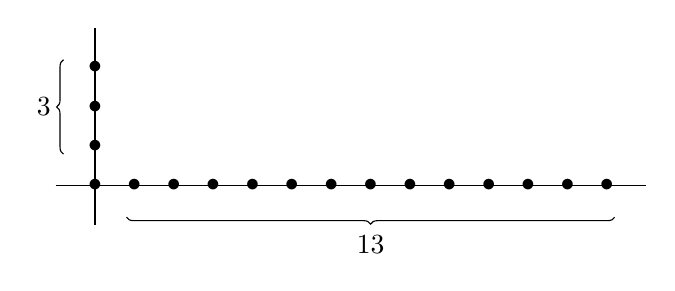
\begin{tikzpicture}[scale = .5]
\node at (0,0) {$\bullet$};
\node at (1,0) {$\bullet$};
\node at (2,0) {$\bullet$};
\node at (3,0) {$\bullet$};
\node at (4,0) {$\bullet$};
\node at (5,0) {$\bullet$};
\node at (6,0) {$\bullet$};
\node at (7,0) {$\bullet$};
\node at (8,0) {$\bullet$};
\node at (9,0) {$\bullet$};
\node at (10,0) {$\bullet$};
\node at (11,0) {$\bullet$};
\node at (12,0) {$\bullet$};
\node at (13,0) {$\bullet$};
\node at (0,1) {$\bullet$};
\node at (0,2) {$\bullet$};
\node at (0,3) {$\bullet$};
\draw (-1,0) -- (14,0);
\draw (0,-1) -- (0,4);
\draw[snake=brace,segment aspect=0.5] (-.8,.8) -- (-.8,3.2);
\draw[snake=brace,segment aspect=0.5] (13.2,-.8) -- (.8,-.8);
\node at (-1.3,2) {$3$};
\node at (7,-1.5) {$13$};
\end{tikzpicture}
\caption{The points $Z$ dual to $\mathcal A_{3,13}$.}
\label{DualA3-13}
\end{center}
\end{figure}

Clearly,  \cite[Propositions 7.2 and 7.4]{DIV} apply to the configuration $\mathcal A_{a,b}$ with $a=3, b=13, d=8$. 
The splitting type in question is $(3,13)$; thus the derivation bundle is unstable.

So we consider the ideal
\[
I = \langle x^8,(x+z)^8,(x+2z)^8,y^8, (y+z)^8,\dots,(y+12z)^8,z^8 \rangle.
\]
Its Hilbert function is 
\[
[1, 3, 6, 10, 15, 21, 28, 36, 33, 27, 19, 12, 7, 3, 1],
\]
as can be verified either on a computer or by hand. For a general linear form $L$, the Hilbert function of $R/(I,L^2)$ is
\[
[1, 3, 5, 7, 9, 11, 13, 15, 5].
\]
Since
\[
[R/I]_{i-2} \stackrel{\times L^2}{\longrightarrow} [R/I]_i \rightarrow [R/(I,L^2)]_i \rightarrow 0
\]
is exact, a comparison of these two Hilbert functions shows that $\times L^2 : [R/I]_{i-2} \rightarrow [R/I]_{i}$ has maximal rank for all $i$. Thus $R/I$ {\em does} have SLP in range 2.

The error seems to be the subtle point that we have studied in this paper, namely the difference between the existence of a curve containing a set of points, with a certain multiplicity at a general point, and the existence of an {\em unexpected} curve with these properties. Applying their proof to this example, they note that $h^0(\mathcal I_Z \otimes I_P^7)(8) \neq 0$, which is true (in fact, the value is 5). But 
\[
5 = h^0((\mathcal I_Z \otimes I_P^7)(8)) = \dim_K [R/(L_1^8,\dots,L_{17}^8,L^2]_8
\]
and 5 is exactly the difference in the dimensions of the components of $R/I$ in degrees 6 and 8, so the failure of surjectivity by 5 is {\em expected} and not an indication that the SLP fails there.
\end{example}

\begin{theorem} \label{SLP condition}
Let $\mathcal A(f)$ be a line arrangement in $\mathbb P^2$, where $f = L_1\cdots L_d$, and let $Z$ be the set of points in $\mathbb P^2$ dual to these lines.  Then $Z$ has an unexpected curve of degree $j$ if and only if $R/(L_1^{j+1},\dots,L_d^{j+1})$ fails the SLP in range 2 and degree $j-1$.
\end{theorem}

\begin{proof}
Let $P$ be a general point in $\mathbb P^2$, and let $L$ be the  linear form dual to $P$. Consider the multiplication map  
\[
\times L^2 : [R/(L_1^{j+1},\dots,L_d^{j+1})]_{j-1} \rightarrow [R/(L_1^{j+1},\dots,L_d^{j+1})]_{j+1}. 
\]
Clearly $\dim_K [R/(L_1^{j+1},\dots,L_d^{j+1})]_{j-1} = \binom{j+1}{2}$. By Macaulay duality, 
\[
\dim_K [R/(L_1^{j+1},\dots,L_d^{j+1})]_{j+1} = h^0(\mathcal I_Z(j+1)).
\]
Hence, the expected dimension of the cokernel is $\max \left \{ h^0(\mathcal I_Z(j+1)) - \binom{j+1}{2}, 0 \right \}$. In other words,  $R/(L_1^{j+1},\dots,L_d^{j+1})$ fails the SLP in range 2 and degree $j-1$ if and only if 
\[
\dim_K (\operatorname{coker} (\times L^2))  > \max \left \{ h^0(\mathcal I_Z(j+1)) - \binom{j+1}{2}, 0 \right \}.
\]

Now, the cokernel of the considered multiplication by $L^2$ is $[R/(L_1^{j+1},\dots,L_d^{j+1},L^2)]_{j+1}$. By Theorem \ref{thm:inverse-system}, its dimension is $h^0((\mathcal I_Z \otimes I_P^{j})(j+1))$. Thus, we have shown that 
$R/(L_1^{j+1},\dots,L_d^{j+1})$ fails the SLP in range 2 and degree $j-1$ if and only if 
\[
h^0((\mathcal I_Z \otimes I_P^{j})(j+1)) > \max \left \{ h^0(\mathcal I_Z(j+1)) - \binom{j+1}{2}, 0 \right \}, 
\]
that is, $Z$ admits an unexpected curve of degree $j+1$. 
\end{proof}

Example \ref{ctrex to DIV} makes it clear that the failure of the syzygy bundle to be stable is not enough to conclude that the ideal $I = (L_1^d,\dots,L_{|Z|}^d)$ fails the SLP at range 2 in any degree. Nevertheless, there is one additional hypothesis that does allow this conclusion.

\begin{corollary} \label{explain DIV}
Let $\mathcal A(f)$ be a line arrangement in $\mathbb P^2$ with splitting type $(a,b)$, where $2 \le a \le b$. Let $f = L_1\cdots L_d$, and let $Z$ be the set of points in $\mathbb P^2$ dual to these lines.  Assume that   $b-a \geq 2$. 
If in addition there is an irreducible curve of degree $a+1$ containing $Z+aP$ then $R/(L_1^{a+1},\dots,L_d^{a+1})$ fails the SLP at range 2 in degree $a-1$. 
\end{corollary}  

\begin{proof}
This follows from Theorem \ref{SLP condition}, via Proposition \ref{gen spec splitting type}, recalling that $a = m_Z$.
\end{proof}

\section{Terao's conjecture} 
\label{sec:Terao}

It is natural to wonder to what extent numerical invariants of a line arrangement are determined by its combinatorial properties. The latter are captured by the \emph{incidence lattice} of the arrangement. It consists of all intersections of lines, ordered by reverse inclusion.  For example, if $\mathcal{A} (f)$ and $\mathcal{A} (g)$  are two line arrangements in ${ \ensuremath{\mathbb{P}}}^2$ with the same incidence lattice, then it follows that the Jacobian ideals of $f$ and $g$ have the same degree. 

One of the main open problems is to decide whether freeness of hyperplane arrangements is a combinatorial property. It is open even for line arrangements. 

\begin{conjecture}[Terao]
    \label{conj:Terao} 
Freeness of a line arrangement  depends  only on its incidence lattice. 
\end{conjecture}

Here we want to use our earlier results to state an equivalent version of this conjecture. We need some preparation. 

Consider a vector bundle $\mathcal{E}$ on ${ \ensuremath{\mathbb{P}}}^2$ of rank two. As pointed out above, its restriction to a general line $L$ has the form 
$\mathcal{O}_L(-a) \oplus \mathcal{O}_L(-b)$ for some integers $a\leq b$. The pair $(a, b)$ is the (generic) \emph{splitting type} of ${\mathcal{E}}$. If $\mathcal E$ splits as a direct sum of line bundles,  then $c_2 ({\mathcal{E}}) = ab$, where $c_2 ({\mathcal{E}})$ denotes the second Chern class of ${\mathcal{E}}$. The converse is true as well. 

\begin{theorem}[{\cite[Theorem 1.45]{Y}}]
  \label{thm:splitt crit}
 For every rank two vector bundle ${\mathcal{E}}$ on ${ \ensuremath{\mathbb{P}}}^2$ with generic splitting type $(a, b)$,  one has $c_2 ({\mathcal{E}}) \ge ab$.  Furthermore, equality is true if and only if ${\mathcal{E}}$ splits as a direct sum of line bundles
\end{theorem} 

Recall that the derivation bundle ${\mathcal{D}} (f)$ of a line arrangement ${\mathcal{A}} (f)$ is the sheafification of the module $D(f)$, defined by the exact sequence 
\[
0 \to D(f) \to R^3 \to \operatorname{Jac} (f) (\deg f -1) \to 0. 
\]
It follows that 
\begin{equation}
   \label{eq:Chern degree} 
   c_2 ({\mathcal{D}} (f) ) = (\deg f - 1)^2 -  \deg \operatorname{Jac} (f). 
\end{equation}

We are ready to establish the following result, which is implicitly used in \cite{DIV}.  

\begin{proposition}
    \label{prop:split type free} 
Let ${\mathcal{A}} (f)$ and ${\mathcal{A}} (g)$ be two line arrangements with the same incidence lattice. Assume ${\mathcal{A}} (f)$ is free with splitting type $(a, b)$. Then one has: 
\begin{itemize}
\item[(a)] ${\mathcal{A}} (g)$ is free if and only if ${\mathcal{D}} (g)$ has the same splitting type as ${\mathcal{D}} (f)$.    

\item[(b)] If ${\mathcal{A}} (g)$ is not free, then the splitting type of ${\mathcal{D}} (g)$ is $(a - s, b+s)$ for some positive integer $s$. 
\end{itemize}
\end{proposition} 

\begin{proof}
Set $d = \deg f$. By Theorem \ref{thm:splitt crit}, since $\mathcal A(f)$ is free we get  $c_2 ({\mathcal{D}} (f)) = ab$.  Since the arrangements have the same incidence lattice, Equation \eqref{eq:Chern degree}  gives $c_2 ({\mathcal{D}} (g)) = c_2 ({\mathcal{D}} (f))$.  Combining, we obtain $c_2 ({\mathcal{D}} (g)) = ab$. 

Since $f$ and $g$ have the same degree, the sum of the integers in the splitting type for ${\mathcal{D}}(f)$ must be equal to the sum for ${\mathcal{D}}(g)$, i.e. the splitting type for ${\mathcal{D}}(g)$ is $(a-s,b+s)$ for some integer $s$, where $a-s \leq b+s$.
Combined with Theorem \ref{thm:splitt crit}, and using the fact that $a+b+1=d$, we obtain 
\[
0 \le c_2 ({\mathcal{D}} (g)) - (a-s) (b+s)  = a b - (a-s) (b+s) = a (d-1-a) - (a-s) (d-1-a+s). 
\]
Since the function $h (t) = t (d-1-t)$ is strictly increasing on the interval $(-\infty, \frac{d-1}{2}]$, and since both $a$ and $a-s$ lie in this interval, we conclude that  $s \ge 0$ and that $c_2 ({\mathcal{D}} (g)) - (a-s) (b+s)  = 0$ if and only if $s = 0$. Hence Theorem \ref{thm:splitt crit} gives that ${\mathcal{D}} (g)$ is free if and only if $s = 0$ and that $s > 0$ otherwise. 
\end{proof}

As an immediate consequence we get: 

\begin{corollary} 
     \label{cor:type of free comb}
If the splitting type of a line arrangement is a combinatorial property  for free arrangements, then Terao's conjecture is true for line arrangements. 
\end{corollary} 

The analogous question is of interest also for non-free arrangements. Thus we propose the following question:

\begin{question}
Is the splitting type a combinatorial invariant for arbitrary arrangements?
\end{question}

Using a Lefschetz-like property, we give a statement that is equivalent to  Terao's conjecture. 

\begin{proposition} 
   \label{prop:Terao equiv} 
The following two conditions are equivalent: 
\begin{itemize}

\item[(a)] Terao's conjecture is true. 

\item[(b)] If ${\mathcal{A}} (f)$ is any free line arrangement with splitting type $(a, b)$, then, for every line arrangement ${\mathcal{A}} (g)$ with the same incidence lattice as ${\mathcal{A}} (f)$, the multiplication map 
\[
[R/J]_{b-2} \stackrel{\times L^2}{\longrightarrow} [R/J]_b
\]
is surjective, where $J = (\ell_1^b,\dots, \ell_{a+b+1}^b, L_1^b,\ldots,L_{b-a}^b)$ with $g = \ell_1 \cdots \ell_{a+b+1}$ and general linear forms $L, L_1,\ldots,L_{b-a} \in R$. 
\end{itemize}
\end{proposition} 

\begin{proof}
Let ${\mathcal{A}} (f)$ be a free line arrangement with splitting type $(a, b)$, and let ${\mathcal{A}} (g)$ be a line arrangement with the same incidence lattice as ${\mathcal{A}} (f)$. By Proposition \ref{prop:split type free}, the splitting type of ${\mathcal{A}} (g)$ is $(a-s, b+s)$ for some integer $s \ge 0$. Let $L, L_1,\ldots,L_{b-a} \in R$ be general linear forms, and set $h = L_1 \cdots L_{b-a}$. Proposition  \ref{prop:change of splitting type} gives  that ${\mathcal{A}} (gh)$ has splitting type $(b-s, b+s)$. Denote by $Z$   the set of points in ${ \ensuremath{\mathbb{P}}}^2$ that is dual to ${\mathcal{A}} (g h)$, and let $P \in { \ensuremath{\mathbb{P}}}^2$  be the point that is dual to $L$. Thus, $Z$ has multiplicity index $m_Z = b -s$ by Theorem~\ref{FVstrong}. 
The cokernel of the 
multiplication map 
\[
[R/J]_{b-2} \stackrel{\times L^2}{\longrightarrow} [R/J]_b
\]
is $[R/(J, L^2)]_b$. By Theorem \ref{thm:inverse-system}, this is isomorphic to $[I_{Z + (b-1)P}]_b$. It follows that the above map is surjective if and only if $m_Z = b$, that is, $s = 0$, which means that   ${\mathcal{A}} (g)$ has the same splitting type as ${\mathcal{A}} (f)$. By Proposition \ref{prop:split type free}, the latter is equivalent to ${\mathcal{A}} (g)$ being free, which concludes the argument. 
\end{proof} 

Similar arguments give a sufficient condition. 

\begin{corollary} 
   \label{cor:suff Terao}
Consider the following condition
\begin{itemize}
\item[(*)] Let $f = \ell'_1 \cdots \ell'_{2k+1}$ and $g =   \ell_1 \cdots \ell_{2k+1}$ be  products of $2k+1$ linear forms in $R$, and let $L \in R$ be a general linear form. Assume that the multiplication map 
\[
[R/I]_{k-2} \stackrel{\times L^2}{\longrightarrow} [R/I]_k
\]
is surjective, where $I = (\ell'^k_1,\dots, \ell'^k_{2k+1})$.  

If the line arrangements ${\mathcal A} (f)$ and ${\mathcal A} (g)$ have the same incidence lattices, then the 
multiplication map 
\[
[R/J]_{k-2} \stackrel{\times L^2}{\longrightarrow} [R/J]_k
\]
is also surjective, where $J =   (\ell_1^k,\dots, \ell_{2k+1}^k)$. 
\end{itemize} 
If Condition (*) is true for any two sets of $2 k+1$ linear forms, then Terao's conjecture is true. 
\end{corollary} 

\begin{proof} 
Adopt the notation of the proof of Proposition \ref{prop:Terao equiv}. In particular, let  ${\mathcal{A}} (f)$ and ${\mathcal{A}} (g)$ be two line arrangements with the same incidence lattice, where ${\mathcal{A}} (f)$ is free with splitting type $(a, b)$.   Let $\ell'_1,\ldots,\ell'_{a+b+1}$ be linear forms such that $f = \ell'_1 \cdots \ell'_{a+b+1}$. We will use Condition (*) by considering the ideal $I = (\ell'^b_1,\dots, \ell'^b_{a+b+1}, L_1^b,\ldots,L_{b-a}^b)$. Indeed, the arrangement ${\mathcal{A}} (f h)$ has splitting type $(b, b)$. Hence the multiplication map 
\[
[R/I]_{b-2} \stackrel{\times L^2}{\longrightarrow} [R/I]_b
\]
is surjective. Since $L_1,\ldots,L_{b-a}$ are general linear forms, the arrangements ${\mathcal{A}} (fh)$ and ${\mathcal{A}} (gh)$ also have the same incidence lattice. Therefore, Condition (*) gives that  the  multiplication map 
\[
[R/J]_{b-2} \stackrel{\times L^2}{\longrightarrow} [R/J]_b
\]
is surjective, where $J =  (\ell^b_1,\dots, \ell^b_{a+b+1}, L_1^b,\ldots,L_{b-a}^b)$. As above, it follows that ${\mathcal{A}} (g)$ must be a free arrangement, as desired. 
\end{proof}

\begin{remark}
(i) In \cite{DIV} the authors conjecture that the above Condition (*) is always satisfied if one replaces surjectivity of the multiplication maps by maximal rank. Moreover, they claim that this modification of Condition (*) is equivalent to Terao's conjecture. 

(ii) We have seen in Example \ref{ctrex to DIV} that injectivity of the multiplication map is not enough to draw a conclusion on the splitting type. One  needs surjectivity as stated in Condition~(*). However, it is not clear (to us) whether Condition (*) is in fact equivalent to Terao's conjecture. 
\end{remark}

\begin{thebibliography}{BNAL}

\bibitem[BGM]{BGM}
A.\ Bigatti, A.\ V. Geramita and J.\ Migliore.
{\it Geometric consequences of extremal behavior in a theorem of Macaulay}.
Trans.\ Amer.\ Math.\ Soc., 346:1 (1994) 203--235.

\bibitem[BM]{BM4} G. Bolondi and J. Migliore, {\it The structure of an even liaison class}, Trans. Amer. Math. Soc. {\bf 316} (1989), 1--37.

\bibitem[Ca]{Camp} 
G.\ Campanella.
{\it Standard bases of perfect homogeneous polynomial ideals of height 2},
J.\  Algebra, 101 (1986) 47--60.

\bibitem[CM]{refCM}
C.\ Ciliberto, R.\ Miranda.
{\it The Segre and Harbourne--Hirschowitz conjectures}, in:
Applications of Algebraic Geometry to Coding Theory, Physics and Computation, 
NATO Sci. Ser. II Math. Phys. Chem., Eilat, 2001, vol. 36, Kluwer Academic, Dordrecht (2001), 37--51.

\bibitem[CHT]{CHT}
S.\ Cooper, B.\ Harbourne and Z.\ Teitler.
{\it Combinatorial bounds on Hilbert functions of fat points in projective space},
J.\ Pure Appl.\ Algebra, 215:9 (2011),  2165--2179.

\bibitem[Da]{Da}
E.\ D.\ Davis.
{\it 0-dimensional subschemes of ${ \ensuremath{\mathbb{P}}}^2$: New application of Castelnuovo's function},
Annali dell'Universitˆ di Ferrara, 1986, Volume 32, Issue 1, 93--107.

\bibitem[DGM]{DGM} 
E.\ D.\ Davis, A.\ V. Geramita and P.\  Maroscia. 
{\it Perfect Homogeneous Ideals: Dubreil's Theorems Revisited}.
Bull.\ Sc.\ math., $2^e$ s\'erie, 108 (1984), 143--185.

\bibitem[DIV]{DIV} 
R.\ Di Gennaro, G.\ Ilardi and J.\ Vall\`es. 
{\it Singular hypersurfaces characterizing the Lefschetz properties}, 
J.\ London Math.\ Soc., (2) 89 (2014), no.\ 1, 194--212 (arXiv:1210.2292).

\bibitem[EI]{EI} 
J.\ Emsalem and A.\ Iarrobino, 
{\it Inverse system of a symbolic power $I$}, 
J.\ Algebra {\bf 174} (1995), 1080--1090.

\bibitem[FV]{FV2} 
D.\ Faenzi and J.\ Vall\`es.
{\it Logarithmic bundles and line arrangements, an approach via the standard construction}, 
J.\ London Math.\ Soc.\ (2) {\bf 90} (2014), 675--694.

\bibitem[GHM]{GHM} 
A.V.\ Geramita, B.\ Harbourne and J.\ Migliore, 
{\it Star configurations in $\mathbb P^n$}, 
J.\ Algebra {\bf 376} (2013), 279--299. 

\bibitem[G]{G}
A.\ Gimigliano,  {\it On linear systems of plane curves}, Thesis, Queen's University, Kingston, 1987.

\bibitem[GM]{GM}
H.\ Grauert  and G.\ M\"ulich, {\it Vektorb\"undel vom Rang 2 \"uber dem $n$-dimensionalen komplex-projektiven Raum},  Manuscripta Math. {\bf 16} (1975), 75--100.

\bibitem[Ha1]{Ha1} 
B.\ Harbourne, 
{\it  The geometry of rational surfaces and Hilbert functions of points in the plane}, Proceedings of
the 1984 Vancouver Conference in Algebraic Geometry, CMS Conf. Proc. {\bf 6},  Amer. Math. Soc., Providence,
RI, (1986) 95--111.

\bibitem[Ha]{Ha} 
B.\ Harbourne, 
{\it Anticanonical rational surfaces}, 
Trans.\ Amer.\ Math.\ Soc.\ 349 (1997) 1191--1208. 

\bibitem[H]{H} 
R.\  Hartshorne, {\it Stable reflexive sheaves},  Math. Ann. {\bf 254} (1980), 121--176.

\bibitem[Hi]{Hi}
A.\ Hirschowitz, {\it Une conjecture pour la cohomologie des diviseurs sur les surfaces rationelles g\'en\'eriques}, J.
Reine Angew. Math. {\bf 397} (1989), 208--213.

\bibitem[HMNW]{HMNW}
T. Harima, J. Migliore, U. Nagel and J. Watanabe, {\em The weak and strong Lefschetz properties for Artinian $K$-algebras}, J. Algebra {\bf 262} (2003), 99--126.

\bibitem[LR]{LR} 
R.\ Lazarsfeld and A.P.\ Rao.
{\it Linkage of general curves of large degree}, 
In: Algebraic geometry -- open problems (Ravello, 1982), LNM 997 (1983), 267--289.

\bibitem[M2]{M2}
D.\ R.\ Grayson and M.\ E.\ Stillman.
{\it Macaulay2, a software system for research in algebraic geometry},
Available at \url{http://www.math.uiuc.edu/Macaulay2/}. 

\bibitem[MN]{MN}
J.\ Migliore  and U.\ Nagel, {\em On the Cohen-Macaulay type of
    the general hypersurface section of a curve},
  Math.\ Z. {\bf 219} (1995), 245--273.

\bibitem[MP]{MP}
J. Migliore and C. Peterson,
{\it A symbolic test for $(i,j)$-uniformity in reduced zero-dimensional schemes}, J. Symbolic Computation {\bf 37} (2004), 403--413.

\bibitem[OSS]{OSS}
C.\ Okonek, M. Schneider, and H.\  Spindler, {\it Vector bundles on complex projective spaces},  Progress in Mathematics {\bf 3},  Birkh\"auser, Boston, Mass., 1980.

\bibitem[OT]{OT} 
P.\ Orlik and H.\ Terao. 
``Arrangement of hyperplanes,'' Grundlehren
der Mathematischen Wissenschaften {\bf 300}, 
Springer-Verlag, Berlin, 1992.

\bibitem[S]{hal} H.\ Schenck. 
{\it Elementary modifications and line configurations in $\mathbb P^2$}, 
Comment.\ Math.\ Helv.\ {\bf 78} (2003), 447--462. 

\bibitem[Se]{segre}
B.\ Segre, {\it Alcune questioni su insiemi finiti di punti in geometria algebrica}, Atti Convegno Intern. di Geom.
Alg. di Torino, (1961), 15--33.

\bibitem[Su]{refSuciu}
A.\ Suciu, {\it Fundamental groups, Alexander invariants, and cohomology jumping loci}, pp.\ 179--223, in:
Contemporary Math., 538, Topology of Algebraic Varieties and Singularities, editors
J.\ I.\ Cogolludo-August\'in, E.\ Hironaka, 2011.

\bibitem[U]{U}
G.\ A.\ Urz\'ua, 
{\it Arrangements of curves and algebraic surfaces},
Thesis (Ph.D.) University of Michigan,  2008. 

\bibitem[Y]{Y}

M.\ Yoshinaga, {\em Freeness of hyperplane arrangements and related topics}, Ann.\ Fac.\ Sci.\ Toulouse Math.\ (6) {\bf 23} (2014), 483--512.

\end{thebibliography}

\end{document}

